\documentclass[12pt,a4paper]{article}
\usepackage[utf8]{inputenc}
\usepackage[T5]{fontenc}
\usepackage[vietnamese]{babel}
\usepackage{mathptmx}           % Times New Roman font
\usepackage{geometry}
\geometry{top=2cm, bottom=2cm, left=2.5cm, right=2cm}
\usepackage{longtable}
\usepackage{array}
\usepackage{amssymb}
\usepackage{indentfirst}
\usepackage{booktabs}
\usepackage{xcolor}
\usepackage{colortbl}
\usepackage{enumitem}
\usepackage{graphicx}
\usepackage{fancyhdr}
\usepackage{lastpage}
\usepackage{tikz}
\usetikzlibrary{calc}

% --- Cấu hình đường dẫn ảnh ---
\graphicspath{{../images/}}

\definecolor{headerblue}{RGB}{220,230,242}
\definecolor{notegreen}{RGB}{234,250,234}

% --- Cấu hình Header & Footer ---
\pagestyle{fancy}
\fancyhf{}
\fancyhead[L]{\small \leftmark}
\fancyhead[R]{\small Trang \thepage/\pageref{LastPage}}
\renewcommand{\headrulewidth}{0.4pt}
\renewcommand{\sectionmark}[1]{\markboth{#1}{}}
\setcounter{tocdepth}{3}
\setcounter{secnumdepth}{3}

\begin{document}

\begin{titlepage}
    \newgeometry{left=2cm, right=2cm, top=2cm, bottom=2cm}
    \begin{tikzpicture}[remember picture, overlay]
        \draw[line width = 2pt] ($(current page.north west) + (1.5cm,-1.5cm)$) rectangle ($(current page.south east) + (-1.5cm,1.5cm)$);
        \draw[line width = 0.5pt] ($(current page.north west) + (1.6cm,-1.6cm)$) rectangle ($(current page.south east) + (-1.6cm,1.6cm)$);
    \end{tikzpicture}

    \begin{center}
        \large \textbf{HỌC VIỆN CÔNG NGHỆ BƯU CHÍNH VIỄN THÔNG} \\
        \large \textbf{KHOA CÔNG NGHỆ THÔNG TIN 2} \\
        \large \textbf{BỘ MÔN THỰC TẬP CƠ SỞ} \\
        \vspace{0.5cm}
        \rule{3cm}{1pt} \\

        \vspace{1.2cm}
        
\includegraphics[width=5.5cm]{Logo_PTIT_University.png} \\
        \vspace{1.5cm}

        \LARGE \textbf{BÁO CÁO CUỐI KỲ} \\
        \vspace{0.5cm}
        \Large \textbf{PHÂN TÍCH VÀ XÁC ĐỊNH YÊU CẦU HỆ THỐNG} \\
        \vspace{1cm}

        \begin{minipage}{14cm}
            \centering
            \large \textbf{Đề tài: Hệ thống nhận diện bệnh trên cây lúa dựa trên thuật toán học sâu CNN}
        \end{minipage}

        \vspace{2.5cm}

        \begin{tabular}{l l}
            \textbf{Giảng viên hướng dẫn:} & Cô Nguyễn Thị Bích Nguyên           \\
            \textbf{Nhóm:}                 & Nhóm 1                              \\
            \textbf{Lớp:}                  & E23CQCE01-N                         \\
            \textbf{Sinh viên thực hiện:}  & 1. Phan Tuấn Quốc Anh - N23DCCN003  \\
                                           & 2. Phạm Minh Khang - N23DCAT034     \\
                                           & 3. Nguyễn Lê Minh Phúc - N23DCDK058 \\
        \end{tabular}

        \vfill
        \large \textbf{TP. HỒ CHÍ MINH - 2026}
    \end{center}
    \restoregeometry
\end{titlepage}

\clearpage
\tableofcontents
\clearpage
\listoffigures
\clearpage
\listoftables
\clearpage

% ============================================================
\section{Tầm nhìn dự án}

\begin{longtable}{|l|p{11.5cm}|}
    \caption{Tầm nhìn dự án}                                                                                                                                 \\
    \hline
    \rowcolor{headerblue}
    \textbf{Mục}               & \textbf{Nội dung}                                                                                                           \\
    \hline
    \textbf{Nỗi đau hiện tại}  & Chẩn đoán bệnh trên cây lúa bằng mắt thường dẫn đến kết quả sai lệch, xử lý chậm trễ (1--3 ngày) và lạm dụng thuốc hóa học. \\
    \hline
    \textbf{Giải pháp đề xuất} & Ứng dụng trí tuệ nhân tạo (CNN) nhận diện bệnh qua hình ảnh, kết hợp dữ liệu thời tiết (GPS) và gợi ý dinh dưỡng thực vật.  \\
    \hline
    \textbf{Giá trị mang lại}  & Chẩn đoán nhanh (5--7 giây), chính xác, giảm phụ thuộc thuốc hóa học, nâng cao năng suất nông nghiệp.                       \\
    \hline
    \textbf{Ngoài phạm vi}     & Cảm biến IoT, thương mại điện tử, tích hợp ERP doanh nghiệp.                                                                \\
    \hline
\end{longtable}

% ============================================================
\section{Quy trình hiện tại và quy trình đề xuất}

\textbf{Quy trình hiện tại (As-Is):}
\begin{enumerate}
    \item Nông dân phát hiện triệu chứng bất thường trên lá lúa.
    \item Tự đoán bệnh dựa trên kinh nghiệm hoặc hỏi người xung quanh (mất 1--3 ngày).
    \item Mua thuốc bảo vệ thực vật theo cảm tính, dễ lạm dụng hóa chất.
\end{enumerate}

\textbf{Quy trình đề xuất (To-Be):}
\begin{enumerate}
    \item Nông dân chụp ảnh lá lúa bằng điện thoại.
    \item Hệ thống AI nhận diện bệnh trong 5--7 giây, khoanh vùng bệnh trên ảnh.
    \item Hệ thống gợi ý dinh dưỡng phù hợp với loại bệnh được phát hiện.
    \item Nông dân có thể phản hồi nếu kết quả chưa chính xác.
    \item Dữ liệu phản hồi được dùng để tái huấn luyện và nâng cấp mô hình AI.
\end{enumerate}

\hrulefill

% ============================================================
\section{Phạm vi áp dụng đề tài}
\begin{itemize}
    \item \textbf{Phạm vi nghiệp vụ:} Hệ thống số hóa quy trình chẩn đoán bệnh lúa qua hình ảnh bằng công nghệ nhận diện chuyên sâu. Hệ thống kết hợp phân tích hình ảnh và các thông số môi trường để đưa ra chẩn đoán chính xác. Kết hợp xây dựng kho tri thức về dinh dưỡng thực vật để gợi ý các loại vitamin và vi lượng cần bổ sung dựa trên việc truy xuất dữ liệu thông minh.
    \item \textbf{Phạm vi đối tượng:} Phục vụ Nông dân (nhận diện \& nhận gợi ý dinh dưỡng) và Quản trị viên (quản lý danh mục, cập nhật mô hình, quản lý kho kiến thức hệ thống).
    \item \textbf{Giới hạn đề tài:} Hệ thống tự chủ kho dữ liệu dinh dưỡng nội bộ. Đối với thông số môi trường, hệ thống sử dụng tọa độ vị trí (GPS) để tự động truy xuất dữ liệu thời tiết làm dữ liệu phụ trợ. Hỗ trợ nhận diện nhiều loại bệnh cùng lúc trên cùng một ảnh.
\end{itemize}

% ============================================================
\section{Các bước xác định yêu cầu}

Quá trình thực hiện xác định yêu cầu gồm 2 bước chính như sau:
\begin{itemize}
    \item \textbf{Bước 1:} Khảo sát hiện trạng, kết quả nhận được là các báo cáo về hiện trạng chẩn đoán bệnh trên cây lúa và nhu cầu bổ sung dinh dưỡng.
    \item \textbf{Bước 2:} Lập danh sách các yêu cầu, kết quả nhận được là danh sách các yêu cầu sẽ được thực hiện trên hệ thống máy tính.
\end{itemize}

\subsection{Đối tượng tham gia xác định yêu cầu}
Gồm 2 nhóm người:
\begin{itemize}
    \item \textbf{Chuyên viên tin học:} Thiết kế kiến trúc nhận diện thông minh, xây dựng kho kiến thức hệ thống và luồng xử lý truy xuất thông tin dinh dưỡng chính xác nhất.
    \item \textbf{Nhà chuyên môn (Kỹ sư nông nghiệp):} Cung cấp dữ liệu ảnh kèm thông số môi trường tương ứng, gán nhãn bệnh và trực tiếp biên soạn/chuẩn hóa bộ dữ liệu văn bản về vitamin/dinh dưỡng.
\end{itemize}
Hai nhóm người này phối hợp thật chặt chẽ để có thể xác định đầy đủ và chính xác các yêu cầu.

\hrulefill

\subsection{Khảo sát hiện trạng}
\subsubsection{Các hình thức thực hiện phổ biến}
\begin{itemize}
    \item \textbf{Quan sát:} Theo dõi và ghi hình quá trình cây lúa biểu hiện triệu chứng thiếu hụt dinh dưỡng hoặc mắc nhiều bệnh cùng lúc trên đồng ruộng dưới các điều kiện thời tiết khác nhau.
    \item \textbf{Khảo sát:} Khảo sát các người nông dân về mối liên hệ giữa các loại bệnh lúa, sự thiếu hụt dinh dưỡng và sự tác động của môi trường (nhiệt độ, độ ẩm).
    \item \textbf{Thu thập thông tin, tài liệu:} Thu thập tập dữ liệu ảnh lá lúa (kèm dữ liệu đặc tả về thời tiết/độ ẩm) và chuẩn bị bộ dữ liệu văn bản về dinh dưỡng thực vật.
\end{itemize}

\subsubsection{Quy trình thực hiện}
\textbf{A. Tìm hiểu tổng quan về thế giới thực:}
\begin{itemize}
    \item Quy mô hoạt động nông nghiệp, các bệnh dịch thường gặp.
    \item Xu hướng chuyển dịch sang bổ sung vitamin tăng sức đề kháng thay vì lạm dụng thuốc hóa học.
\end{itemize}

\textbf{B. Tìm hiểu hiện trạng tổ chức (cơ cấu tổ chức):}
\begin{itemize}
    \item Cơ cấu tổ chức bao gồm các chức danh: Quản trị viên (Quản lý dữ liệu bệnh, mô hình, tập dữ liệu dinh dưỡng), Nông dân (tải ảnh và mô tả tình trạng).
\end{itemize}

\textbf{C. Tìm hiểu hiện trạng nghiệp vụ:}
\begin{itemize}
    \item Việc tìm hiểu dựa trên: Thông tin đầu vào, Quá trình xử lý, Thông tin kết xuất.
    \item Xếp loại các nghiệp vụ vào 4 loại: Lưu trữ, Tính toán, Tra cứu, Kết xuất.
\end{itemize}

\hrulefill

\subsection{Lập danh sách các yêu cầu}
\subsubsection{Xác định yêu cầu chức năng nghiệp vụ}

% ============================================================
% NGƯỜI DÙNG: NÔNG DÂN
% ============================================================
\section{Người dùng --- Nông dân (Mã số: ND)}

\textbf{Định nghĩa:} Người sử dụng hệ thống với mục đích chẩn đoán bệnh trên cây lúa qua hình ảnh, xem gợi ý dinh dưỡng và phản hồi kết quả chẩn đoán.

\vspace{0.3cm}
\textbf{1. Bảng yêu cầu chức năng nghiệp vụ}

\begin{longtable}{|c|l|l|l|l|p{3.5cm}|}
    \hline
    \rowcolor{headerblue}
    \textbf{STT} & \textbf{Công việc}               & \textbf{Loại công việc} & \textbf{Quy định/CT liên quan} & \textbf{Biểu mẫu liên quan} & \textbf{Ghi chú}         \\
    \hline
    \endhead
    \multicolumn{6}{|l|}{\cellcolor{notegreen}\textbf{I. Quản lý tài khoản}}                                                                                            \\
    \hline
    1            & Đăng ký tài khoản                & Lưu trữ                 & QĐ-ND-01                       & ND\_BM 1                    &                          \\
    \hline
    2            & Đăng nhập hệ thống               & Tra cứu                 & QĐ-ND-01                       &                             &                          \\
    \hline
    3            & Khôi phục mật khẩu               & Lưu trữ                 & QĐ-ND-01                       &                             &                          \\
    \hline
    \multicolumn{6}{|l|}{\cellcolor{notegreen}\textbf{II. Hồ sơ cá nhân}}                                                                                               \\
    \hline
    4            & Xem thông tin cá nhân            & Tra cứu                 & QĐ-ND-02                       &                             &                          \\
    \hline
    5            & Chỉnh sửa thông tin cá nhân      & Lưu trữ                 & QĐ-ND-02                       & ND\_BM 2                    &                          \\
    \hline
    \multicolumn{6}{|l|}{\cellcolor{notegreen}\textbf{III. Chẩn đoán bệnh lúa}}                                                                                         \\
    \hline
    6            & Gửi ảnh lúa để chẩn đoán         & Lưu trữ                 & QĐ-ND-03                       & ND\_BM 3                    &                          \\
    \hline
    7            & Nhập thông số môi trường bổ sung & Lưu trữ                 & QĐ-ND-03                       &                             & Tùy chọn, không bắt buộc \\
    \hline
    8            & Xem kết quả chẩn đoán            & Tra cứu, Tính toán      & QĐ-ND-03                       &                             &                          \\
    \hline
    \multicolumn{6}{|l|}{\cellcolor{notegreen}\textbf{IV. Tra cứu \& Phản hồi}}                                                                                         \\
    \hline
    9            & Tra cứu lịch sử chẩn đoán        & Tra cứu                 & QĐ-ND-04                       &                             &                          \\
    \hline
    10           & Xem chi tiết một lần chẩn đoán   & Tra cứu                 & QĐ-ND-04                       &                             &                          \\
    \hline
    11           & Gửi phản hồi kết quả             & Lưu trữ                 & QĐ-ND-05                       & ND\_BM 4                    &                          \\
    \hline
    12           & Xem kết quả xử lý phản hồi       & Tra cứu                 & QĐ-ND-05                       &                             &                          \\
    \hline
\end{longtable}

% ============================================================
\vspace{0.3cm}
\textbf{2. Bảng Quy định / Công thức liên quan --- Nông dân}

\begin{longtable}{|c|l|l|p{7cm}|l|}
    \hline
    \rowcolor{headerblue}
    \textbf{STT} & \textbf{Mã số} & \textbf{Tên Quy định}      & \textbf{Mô tả chi tiết}                                                                                                                                     & \textbf{Ghi chú} \\
    \hline
    \endhead
    1            & QĐ-ND-01       & Quy định Quản lý tài khoản & Bao gồm quy trình đăng ký (có xác thực email), đăng nhập (kiểm tra cặp tên đăng nhập + mật khẩu, khóa sau 5 lần sai) và khôi phục mật khẩu (OTP qua email). &                  \\
    \hline
    2            & QĐ-ND-02       & Quy định Hồ sơ cá nhân     & Bao gồm quy trình xem và chỉnh sửa thông tin cá nhân. Chỉ được sửa họ tên hiển thị và vị trí GPS. Tên đăng nhập và email không thay đổi.                    &                  \\
    \hline
    3            & QĐ-ND-03       & Quy định Chẩn đoán bệnh    & Bao gồm quy trình gửi ảnh chẩn đoán, nhập thông số môi trường bổ sung (tùy chọn) và xem kết quả chẩn đoán kèm gợi ý dinh dưỡng.                             &                  \\
    \hline
    4            & QĐ-ND-04       & Quy định Tra cứu lịch sử   & Bao gồm quy trình tra cứu danh sách lịch sử chẩn đoán và xem chi tiết một lần chẩn đoán cụ thể.                                                             &                  \\
    \hline
    5            & QĐ-ND-05       & Quy định Phản hồi kết quả  & Bao gồm quy trình gửi phản hồi về kết quả chẩn đoán và xem kết quả xử lý phản hồi từ quản trị viên.                                                         &                  \\
    \hline
\end{longtable}

% ============================================================
\vspace{0.3cm}
\textbf{3. Chi tiết từng Quy định --- Nông dân}

\vspace{0.3cm}
\noindent\textbf{QĐ-ND-01 --- Quy định Quản lý tài khoản}

\noindent\textit{a) Đăng ký tài khoản}

\noindent\textbf{Định nghĩa:} Tài khoản bao gồm 4 thông tin: tên đăng nhập, địa chỉ email, mật khẩu và xác nhận mật khẩu.

\noindent\textbf{Quy trình đăng ký:}
\begin{enumerate}
    \item Người dùng nhập đầy đủ 4 thông tin trên.
    \item Hệ thống kiểm tra tính hợp lệ: tên đăng nhập chưa tồn tại, email chưa được đăng ký, mật khẩu đủ mạnh (tối thiểu 8 ký tự, gồm chữ hoa, chữ số và ký tự đặc biệt), xác nhận mật khẩu khớp.
    \item Hệ thống tạo tài khoản ở trạng thái \textbf{chưa kích hoạt} và gửi email xác thực chứa liên kết kích hoạt.
    \item Người dùng nhấn liên kết trong email để \textbf{kích hoạt tài khoản}.
    \item Sau khi kích hoạt, người dùng có thể đăng nhập vào hệ thống.
\end{enumerate}

\noindent\textit{b) Đăng nhập hệ thống}

\noindent\textbf{Quy trình đăng nhập:}
\begin{enumerate}
    \item Người dùng nhập 2 thông tin: tên đăng nhập (hoặc email) và mật khẩu.
    \item Hệ thống kiểm tra mật khẩu có đúng với tên đăng nhập hoặc email đã nhập hay không.
    \item Nếu sai, hệ thống thông báo chung ``Tên đăng nhập hoặc mật khẩu không chính xác''. Nhập sai 5 lần liên tiếp thì khóa tài khoản 15 phút.
    \item Nếu đúng và tài khoản đã kích hoạt, đăng nhập thành công.
\end{enumerate}

\noindent\textit{c) Khôi phục mật khẩu}

\noindent\textbf{Quy trình khôi phục:}
\begin{enumerate}
    \item Nhập \textbf{địa chỉ email} đã đăng ký trong hệ thống.
    \item Hệ thống gửi \textbf{mã OTP} 6 chữ số về email --- hiệu lực 10 phút. Nhập sai 3 lần thì hủy mã.
    \item Nhập \textbf{mật khẩu mới} --- không được trùng mật khẩu cũ, đáp ứng độ mạnh như khi đăng ký.
    \item Nhập \textbf{xác nhận mật khẩu mới} --- phải gõ chính xác giống bước 3.
\end{enumerate}

\vspace{0.3cm}
\noindent\textbf{QĐ-ND-02 --- Quy định Hồ sơ cá nhân}

\noindent\textit{a) Xem thông tin cá nhân}

Người dùng chỉ xem được thông tin của chính mình sau khi đã đăng nhập. Thông tin hiển thị gồm: tên đăng nhập, họ tên, địa chỉ email, vị trí GPS và ngày tham gia hệ thống.

\noindent\textit{b) Chỉnh sửa thông tin cá nhân}

\noindent\textbf{Định nghĩa:} Hồ sơ cá nhân gồm 2 thông tin được phép sửa: họ tên hiển thị và vị trí GPS.

\noindent\textbf{Quy trình chỉnh sửa:}
\begin{enumerate}
    \item Người dùng chỉnh sửa họ tên hiển thị hoặc kéo thả ghim trên bản đồ để cập nhật vị trí GPS mặc định.
    \item Hệ thống cập nhật thông tin và thông báo thành công.
\end{enumerate}
\noindent\textbf{Ràng buộc:} Tên đăng nhập và địa chỉ email không được phép thay đổi.

\vspace{0.3cm}
\noindent\textbf{QĐ-ND-03 --- Quy định Chẩn đoán bệnh}

\noindent\textit{a) Gửi ảnh chẩn đoán}

\noindent\textbf{Quy trình gửi ảnh:}
\begin{enumerate}
    \item Người dùng chọn ảnh lá lúa (định dạng JPG hoặc PNG, dung lượng tối đa 10MB).
    \item Hệ thống tự động lấy tọa độ GPS từ hồ sơ để truy xuất dữ liệu thời tiết phục vụ chẩn đoán.
    \item Hệ thống gửi ảnh đến mô hình AI để nhận diện bệnh.
\end{enumerate}

\noindent\textit{b) Nhập thông số môi trường bổ sung} \textit{(tùy chọn)}

Không bắt buộc. Người dùng có thể cung cấp thêm vị trí hiện tại (kéo thả ghim trên bản đồ nếu khác với vị trí trong hồ sơ) và mô tả tình trạng ruộng lúa thực tế. Nếu cung cấp, hệ thống sẽ dùng để điều chỉnh kết quả chẩn đoán.

\noindent\textit{c) Xem kết quả chẩn đoán}

Hệ thống hiển thị kết quả gồm: tên bệnh được chẩn đoán, vùng bệnh khoanh trực tiếp trên ảnh gốc, phần trăm độ tin cậy và gợi ý dinh dưỡng tương ứng.

\vspace{0.3cm}
\noindent\textbf{QĐ-ND-04 --- Quy định Tra cứu lịch sử}

\noindent\textit{a) Tra cứu lịch sử chẩn đoán}

\noindent\textbf{Quy trình tra cứu:}
\begin{enumerate}
    \item Người dùng lọc lịch sử theo khoảng thời gian (từ ngày --- đến ngày) hoặc theo tên bệnh cụ thể.
    \item Hệ thống hiển thị danh sách lịch sử chẩn đoán của chính người đang đăng nhập, 10 dòng mỗi trang.
\end{enumerate}

\noindent\textit{b) Xem chi tiết một lần chẩn đoán}

Hệ thống hiển thị đầy đủ thông tin gồm: ảnh gốc, vùng khoanh bệnh, tên bệnh, độ tin cậy và gợi ý dinh dưỡng tương ứng.

\vspace{0.3cm}
\noindent\textbf{QĐ-ND-05 --- Quy định Phản hồi kết quả}

\noindent\textit{a) Gửi phản hồi kết quả}

\noindent\textbf{Quy trình gửi phản hồi:}
\begin{enumerate}
    \item Người dùng chọn tên bệnh thực tế từ danh sách có sẵn. Nếu chọn ``Khác'' thì nhập tên bệnh vào ô trống.
    \item Nhập lời nhắn kèm theo (không bắt buộc).
    \item Gửi phiếu phản hồi --- phiếu ở trạng thái ``Chờ xử lý'' và không được phép chỉnh sửa sau khi gửi.
\end{enumerate}

\noindent\textit{b) Xem kết quả xử lý phản hồi}

Hệ thống hiển thị thông tin gồm: trạng thái phiếu (Chờ xử lý / Chấp nhận / Từ chối), tên quản trị viên xử lý và lời nhắn phản hồi từ quản trị viên.

% ============================================================
\vspace{0.3cm}
\textbf{4. Các Biểu mẫu --- Nông dân}

\vspace{0.3cm}
\noindent\textbf{ND\_BM 1: PHIẾU ĐĂNG KÝ TÀI KHOẢN}

\noindent Tên đăng nhập: \dotfill \\
Địa chỉ email: \dotfill \\
Mật khẩu: \dotfill \\
Xác nhận mật khẩu: \dotfill

\vspace{0.3cm}
\noindent\textbf{ND\_BM 2: PHIẾU CHỈNH SỬA THÔNG TIN CÁ NHÂN}

\noindent Tên đăng nhập: \dotfill \textit{(không được sửa)} \\
Địa chỉ email: \dotfill \textit{(không được sửa)} \\
Họ tên hiển thị: \dotfill \\
Vị trí GPS: [Bản đồ] \textit{(kéo thả ghim để cập nhật)}

\vspace{0.3cm}
\noindent\textbf{ND\_BM 3: PHIẾU GỬI ẢNH CHẨN ĐOÁN}

\noindent Ảnh lá lúa: [Chọn file] \textit{(JPG/PNG, tối đa 10MB)} \\
Vị trí GPS hiện tại: \dotfill \textit{(tự động lấy từ hồ sơ)} \\
Thông số môi trường bổ sung: [Xem ND\_BM 3b] \textit{(tùy chọn)}

\vspace{0.2cm}
\noindent\textbf{ND\_BM 3b: PHIẾU NHẬP THÔNG SỐ MÔI TRƯỜNG} \textit{(tùy chọn)}

\noindent Vị trí hiện tại: [Bản đồ] \textit{(kéo thả ghim nếu khác hồ sơ)} \\
Mô tả thực tế: \dotfill \\
\dotfill \\
\textit{(Ví dụ: ngập úng, sương mù, ruộng mới phun thuốc...)}

\vspace{0.3cm}
\noindent\textbf{ND\_BM 4: PHIẾU PHẢN HỒI KẾT QUẢ CHẨN ĐOÁN}

\noindent Mã chẩn đoán: \dotfill \quad Ngày gửi: \dotfill \\
AI chẩn đoán: \dotfill \quad Độ tin cậy: \dots\% \\
Loại bệnh thực tế: [Danh sách chọn] \textit{(nếu chọn ``Khác'' thì nhập tên bệnh: \dotfill)} \\
Lời nhắn kèm theo: \dotfill \\
\dotfill

% ============================================================
% NGƯỜI DÙNG: QUẢN TRỊ VIÊN
% ============================================================
\section{Người dùng --- Quản trị viên (Mã số: AD)}

\textbf{Định nghĩa:} Người sử dụng hệ thống với mục đích quản lý danh mục bệnh lúa, kho tri thức dinh dưỡng, tài khoản người dùng và theo dõi hiệu suất mô hình AI.

\vspace{0.3cm}
\textbf{1. Bảng yêu cầu chức năng nghiệp vụ}

\begin{longtable}{|c|l|l|l|l|p{3.5cm}|}
    \hline
    \rowcolor{headerblue}
    \textbf{STT} & \textbf{Công việc}          & \textbf{Loại công việc} & \textbf{Quy định/CT liên quan} & \textbf{Biểu mẫu liên quan} & \textbf{Ghi chú} \\
    \hline
    \endhead
    \multicolumn{6}{|l|}{\cellcolor{notegreen}\textbf{I. Tài khoản quản trị}}                                                                              \\
    \hline
    1            & Đăng nhập hệ thống quản trị & Tra cứu                 & QĐ-AD-01                       &                             &                  \\
    \hline
    2            & Đổi mật khẩu quản trị       & Lưu trữ                 & QĐ-AD-01                       &                             &                  \\
    \hline
    \multicolumn{6}{|l|}{\cellcolor{notegreen}\textbf{II. Quản lý bệnh lúa}}                                                                               \\
    \hline
    3            & Quản lý bệnh lúa            & Lưu trữ                 & QĐ-AD-02                       & AD\_BM 1                    &                  \\
    \hline
    \multicolumn{6}{|l|}{\cellcolor{notegreen}\textbf{III. Quản lý tri thức dinh dưỡng}}                                                                   \\
    \hline
    4            & Quản lý tri thức dinh dưỡng & Lưu trữ                 & QĐ-AD-03                       & AD\_BM 2                    &                  \\
    \hline
    \multicolumn{6}{|l|}{\cellcolor{notegreen}\textbf{IV. Quản lý người dùng}}                                                                             \\
    \hline
    5            & Xem danh sách người dùng    & Tra cứu                 & QĐ-AD-04                       &                             &                  \\
    \hline
    6            & Khóa / Mở khóa tài khoản    & Lưu trữ                 & QĐ-AD-04                       &                             &                  \\
    \hline
    \multicolumn{6}{|l|}{\cellcolor{notegreen}\textbf{V. Quản lý phản hồi}}                                                                                \\
    \hline
    7            & Xem danh sách phản hồi      & Tra cứu                 & QĐ-AD-05                       &                             &                  \\
    \hline
    8            & Xử lý phản hồi              & Lưu trữ                 & QĐ-AD-05                       & AD\_BM 3                    &                  \\
    \hline
    \multicolumn{6}{|l|}{\cellcolor{notegreen}\textbf{VI. Hệ thống}}                                                                                       \\
    \hline
    9            & Cập nhật mô hình AI         & Lưu trữ                 & QĐ-AD-06                       &                             &                  \\
    \hline
    10           & Xem thống kê \& báo cáo     & Tra cứu, Kết xuất       & QĐ-AD-06                       & AD\_BM 4                    &                  \\
    \hline
\end{longtable}

% ============================================================
\vspace{0.3cm}
\textbf{2. Bảng Quy định / Công thức liên quan --- Quản trị viên}

\begin{longtable}{|c|l|l|p{7.5cm}|l|}
    \hline
    \rowcolor{headerblue}
    \textbf{STT} & \textbf{Mã số} & \textbf{Tên Quy định}                & \textbf{Mô tả chi tiết}                                                                                                & \textbf{Ghi chú} \\
    \hline
    \endhead
    1            & QĐ-AD-01       & Quy định Tài khoản quản trị          & Bao gồm quy trình đăng nhập (kiểm tra cặp tên đăng nhập + mật khẩu, khóa sau 5 lần sai trong 30 phút) và đổi mật khẩu. &                  \\
    \hline
    2            & QĐ-AD-02       & Quy định Quản lý bệnh lúa            & Bao gồm quy trình thêm, sửa, ẩn/xóa bệnh lúa. Tên bệnh duy nhất, xóa vĩnh viễn chỉ khi chưa có lịch sử.                &                  \\
    \hline
    3            & QĐ-AD-03       & Quy định Quản lý tri thức dinh dưỡng & Bao gồm quy trình thêm, sửa, xóa thông tin dinh dưỡng. Mỗi bản ghi phải gắn với một loại bệnh cụ thể.                  &                  \\
    \hline
    4            & QĐ-AD-04       & Quy định Quản lý người dùng          & Bao gồm quy trình xem danh sách người dùng và khóa/mở khóa tài khoản. Admin không được chỉnh sửa thông tin người dùng. &                  \\
    \hline
    5            & QĐ-AD-05       & Quy định Xử lý phản hồi              & Bao gồm quy trình xem danh sách phiếu phản hồi, xem xét kết quả và chốt trạng thái xử lý.                              &                  \\
    \hline
    6            & QĐ-AD-06       & Quy định Hệ thống                    & Bao gồm quy trình cập nhật mô hình AI và xem thống kê/báo cáo hiệu suất.                                               &                  \\
    \hline
\end{longtable}

% ============================================================
\vspace{0.3cm}
\textbf{3. Chi tiết từng Quy định --- Quản trị viên}

\vspace{0.3cm}
\noindent\textbf{QĐ-AD-01 --- Quy định Tài khoản quản trị}

\noindent\textit{a) Đăng nhập hệ thống quản trị}

\noindent\textbf{Quy trình đăng nhập:}
\begin{enumerate}
    \item Quản trị viên nhập 2 thông tin: tên đăng nhập và mật khẩu.
    \item Hệ thống kiểm tra mật khẩu có đúng với tên đăng nhập đã nhập hay không.
    \item Nếu sai, hệ thống thông báo chung ``Tên đăng nhập hoặc mật khẩu không chính xác''. Nhập sai 5 lần liên tiếp thì khóa tài khoản 30 phút.
    \item Nếu đúng, đăng nhập thành công vào trang quản trị.
\end{enumerate}

\noindent\textit{b) Đổi mật khẩu}

\noindent\textbf{Quy trình đổi mật khẩu:}
\begin{enumerate}
    \item Nhập mật khẩu hiện tại để xác thực.
    \item Nhập mật khẩu mới --- phải đáp ứng độ mạnh (tối thiểu 8 ký tự, gồm chữ hoa, chữ số và ký tự đặc biệt) và không được trùng mật khẩu cũ.
    \item Nhập xác nhận mật khẩu mới --- phải gõ chính xác giống bước 2.
\end{enumerate}

\vspace{0.3cm}
\noindent\textbf{QĐ-AD-02 --- Quy định Quản lý bệnh lúa}

\noindent\textbf{Định nghĩa:} Bản ghi bệnh lúa gồm 3 thông tin: tên bệnh (tiếng Việt), tên khoa học và mô tả triệu chứng.

\noindent\textbf{Quy trình quản lý:}
\begin{enumerate}
    \item \textbf{Thêm bệnh:} Nhập đầy đủ 3 thông tin. Tên bệnh và tên khoa học phải là duy nhất trong hệ thống.
    \item \textbf{Sửa bệnh:} Chỉnh sửa thông tin bệnh nhưng không được thay đổi mã định danh hệ thống.
    \item \textbf{Xóa / Ẩn bệnh:} Nếu bệnh chưa có dữ liệu lịch sử chẩn đoán thì xóa vĩnh viễn. Nếu đã có lịch sử thì chỉ được chuyển sang trạng thái ``Ẩn''.
\end{enumerate}

\vspace{0.3cm}
\noindent\textbf{QĐ-AD-03 --- Quy định Quản lý tri thức dinh dưỡng}

\noindent\textbf{Định nghĩa:} Bản ghi dinh dưỡng gồm: bệnh lúa áp dụng (bắt buộc), nội dung tri thức (hoạt chất, hướng dẫn sử dụng).

\noindent\textbf{Quy trình quản lý:}
\begin{enumerate}
    \item \textbf{Thêm:} Chọn bệnh lúa từ danh mục, nhập nội dung tri thức. Mỗi bản ghi phải gắn với một loại bệnh cụ thể.
    \item \textbf{Sửa:} Cập nhật nội dung tri thức. Hệ thống tự động cập nhật dữ liệu tìm kiếm ngữ nghĩa.
    \item \textbf{Xóa:} Xóa bản ghi khỏi kho tri thức. Thay đổi có hiệu lực ngay lập tức.
\end{enumerate}

\vspace{0.3cm}
\noindent\textbf{QĐ-AD-04 --- Quy định Quản lý người dùng}

\noindent\textit{a) Xem danh sách người dùng}

Hệ thống hiển thị danh sách người dùng với thông tin định danh: tên đăng nhập, email, số lượt chẩn đoán, số lượt phản hồi và trạng thái tài khoản.

\noindent\textit{b) Khóa / Mở khóa tài khoản}

\noindent\textbf{Quy trình:}
\begin{enumerate}
    \item Quản trị viên chọn tài khoản cần thay đổi trạng thái.
    \item Chuyển trạng thái giữa ``Hoạt động'' và ``Tạm khóa''.
\end{enumerate}
\noindent\textbf{Ràng buộc:} Quản trị viên không được chỉnh sửa tên đăng nhập, email hoặc bất kỳ thông tin cá nhân nào của người dùng.

\vspace{0.3cm}
\noindent\textbf{QĐ-AD-05 --- Quy định Xử lý phản hồi}

\noindent\textbf{Quy trình xử lý:}
\begin{enumerate}
    \item Xem danh sách phiếu chưa xử lý, ưu tiên phiếu gửi sớm nhất.
    \item Xem xét song song: ảnh gốc, kết quả AI và kết quả nông dân báo cáo.
    \item Nhập lời nhắn phản hồi gửi lại cho nông dân.
    \item Chốt trạng thái xử lý: ``Chấp nhận'' (AI sai) hoặc ``Từ chối'' (AI đúng).
\end{enumerate}
\noindent\textbf{Ràng buộc:} Nếu chọn ``Chấp nhận'', hệ thống tự động lưu ảnh vào tập dữ liệu để nâng cấp mô hình AI sau này.

\vspace{0.3cm}
\noindent\textbf{QĐ-AD-06 --- Quy định Hệ thống}

\noindent\textit{a) Cập nhật mô hình AI}

\noindent\textbf{Quy trình cập nhật:}
\begin{enumerate}
    \item Tải lên file mô hình AI mới kèm tên phiên bản và ghi chú thay đổi.
    \item Hệ thống lưu file mô hình ở trạng thái chưa kích hoạt.
    \item Quản trị viên dùng công tắc ``Kích hoạt'' để áp dụng mô hình mới cho toàn hệ thống. Mô hình cũ tự động tắt.
\end{enumerate}

\noindent\textit{b) Thống kê \& Báo cáo}

Hệ thống hiển thị 2 loại báo cáo:
\begin{itemize}
    \item \textbf{Bản đồ dịch bệnh:} bản đồ nhiệt tình hình dịch bệnh theo tọa độ GPS của các ca chẩn đoán.
    \item \textbf{Hiệu suất AI:} thống kê tỷ lệ chẩn đoán đúng/sai theo từng loại bệnh dựa trên kết quả xử lý phản hồi.
\end{itemize}

% ============================================================
\vspace{0.3cm}
\textbf{4. Các Biểu mẫu --- Quản trị viên}

\vspace{0.3cm}
\noindent\textbf{AD\_BM 1: PHIẾU QUẢN LÝ BỆNH LÚA}

\noindent Tên bệnh: \dotfill \\
Tên khoa học: \dotfill \\
Mô tả triệu chứng: \dotfill \\
\dotfill \\
Trạng thái: $\square$ Hiển thị \quad $\square$ Ẩn

\vspace{0.3cm}
\noindent\textbf{AD\_BM 2: PHIẾU QUẢN LÝ TRI THỨC DINH DƯỠNG}

\noindent Bệnh lúa áp dụng: [Danh sách chọn] \dotfill \\
Hoạt chất bổ sung: \dotfill \\
Hướng dẫn sử dụng: \dotfill \\
\dotfill

\vspace{0.3cm}
\noindent\textbf{AD\_BM 3: PHIẾU XỬ LÝ PHẢN HỒI}

\noindent Mã phản hồi: \dotfill \quad Người dùng gửi: \dotfill \\
Ảnh gốc: [Hiển thị ảnh lá lúa] \\
AI chẩn đoán: \dotfill \quad Độ tin cậy: \dots\% \\
Nông dân báo cáo: \dotfill \\
Lời nhắn của nông dân: \dotfill \\
Trạng thái xử lý: $\square$ Chấp nhận (AI sai) \quad $\square$ Từ chối (AI đúng) \\
Lời nhắn phản hồi: \dotfill \\
\dotfill

\vspace{0.3cm}
\noindent\textbf{AD\_BM 4: BÁO CÁO HIỆU SUẤT AI}

\noindent Tháng: \dotfill \quad Năm: \dotfill

\begin{longtable}{|c|l|p{4cm}|p{3cm}|p{3cm}|}
    \hline
    \rowcolor{headerblue}
    \textbf{STT} & \textbf{Mã bệnh} & \textbf{Tên bệnh} & \textbf{Số lượt nhận diện} & \textbf{Số lượt AI đoán sai} \\
    \hline
    1            &                  &                   &                            &                              \\
    \hline
    2            &                  &                   &                            &                              \\
    \hline
    3            &                  &                   &                            &                              \\
    \hline
\end{longtable}
\noindent Ngày lập báo cáo: \dotfill \quad Người lập: \dotfill

\hrulefill

% ============================================================
\subsubsection{Xác định yêu cầu chức năng hệ thống và yêu cầu chất lượng}

\textbf{Bảng yêu cầu chức năng hệ thống:}
\begin{longtable}{|c|l|p{9.5cm}|l|}
    \hline
    \rowcolor{headerblue}
    \textbf{STT} & \textbf{Nội dung}  & \textbf{Mô tả chi tiết}                                                                            & \textbf{Ghi chú} \\
    \hline
    \endhead
    1            & Tích hợp thời tiết & Truy xuất dữ liệu thời tiết dựa trên tọa độ thực tế của nông dân để cung cấp bối cảnh môi trường.  &                  \\
    \hline
    2            & Quản lý tri thức   & Hệ thống đồng bộ các hướng dẫn dinh dưỡng để AI có thể tư vấn linh hoạt.                           &                  \\
    \hline
    3            & Bảo mật dữ liệu    & Mật khẩu được bảo mật an toàn. Toàn bộ ảnh và dữ liệu thực tế được lưu trữ phục vụ tái huấn luyện. &                  \\
    \hline
    4            & Gửi mã xác thực    & Tự động gửi mã xác thực qua email cho các luồng xác minh tài khoản.                                &                  \\
    \hline
\end{longtable}

\textbf{Bảng yêu cầu về chất lượng hệ thống:}
\begin{longtable}{|c|l|l|p{6.5cm}|l|}
    \hline
    \rowcolor{headerblue}
    \textbf{STT} & \textbf{Nội dung} & \textbf{Tiêu chuẩn} & \textbf{Mô tả chi tiết}                                                    & \textbf{Ghi chú} \\
    \hline
    \endhead
    1            & Cập nhật mô hình  & Tiến hóa            & Có thể thay thế mô hình nhận diện mới mà không làm gián đoạn người dùng.   &                  \\
    \hline
    2            & Tính tiện dụng    & Tiện dụng           & Giao diện tối ưu cho thiết bị di động, thông báo rõ ràng bằng tiếng Việt.  &                  \\
    \hline
    3            & Tốc độ xử lý      & Hiệu quả            & Phản hồi kết quả chẩn đoán trong vòng 5--7 giây.                           &                  \\
    \hline
    4            & Độ tương thích    & Tương thích         & Hoạt động ổn định trên các trình duyệt phổ biến của điện thoại thông minh. &                  \\
    \hline
    5            & Tính kịp thời     & Hiệu quả            & Mã xác thực gửi đến người dùng trong vòng 30 giây.                         &                  \\
    \hline
\end{longtable}

\hrulefill

% ============================================================
\section{Biểu đồ Use Case}

\subsection{Biểu đồ Use Case --- Nông dân}

% Chèn ảnh Use Case Nông dân (xuất từ Mermaid/draw.io)
% \noindent\textit{[Chèn ảnh Use Case Nông dân tại đây]}
\begin{figure}[htbp]
    \centering
    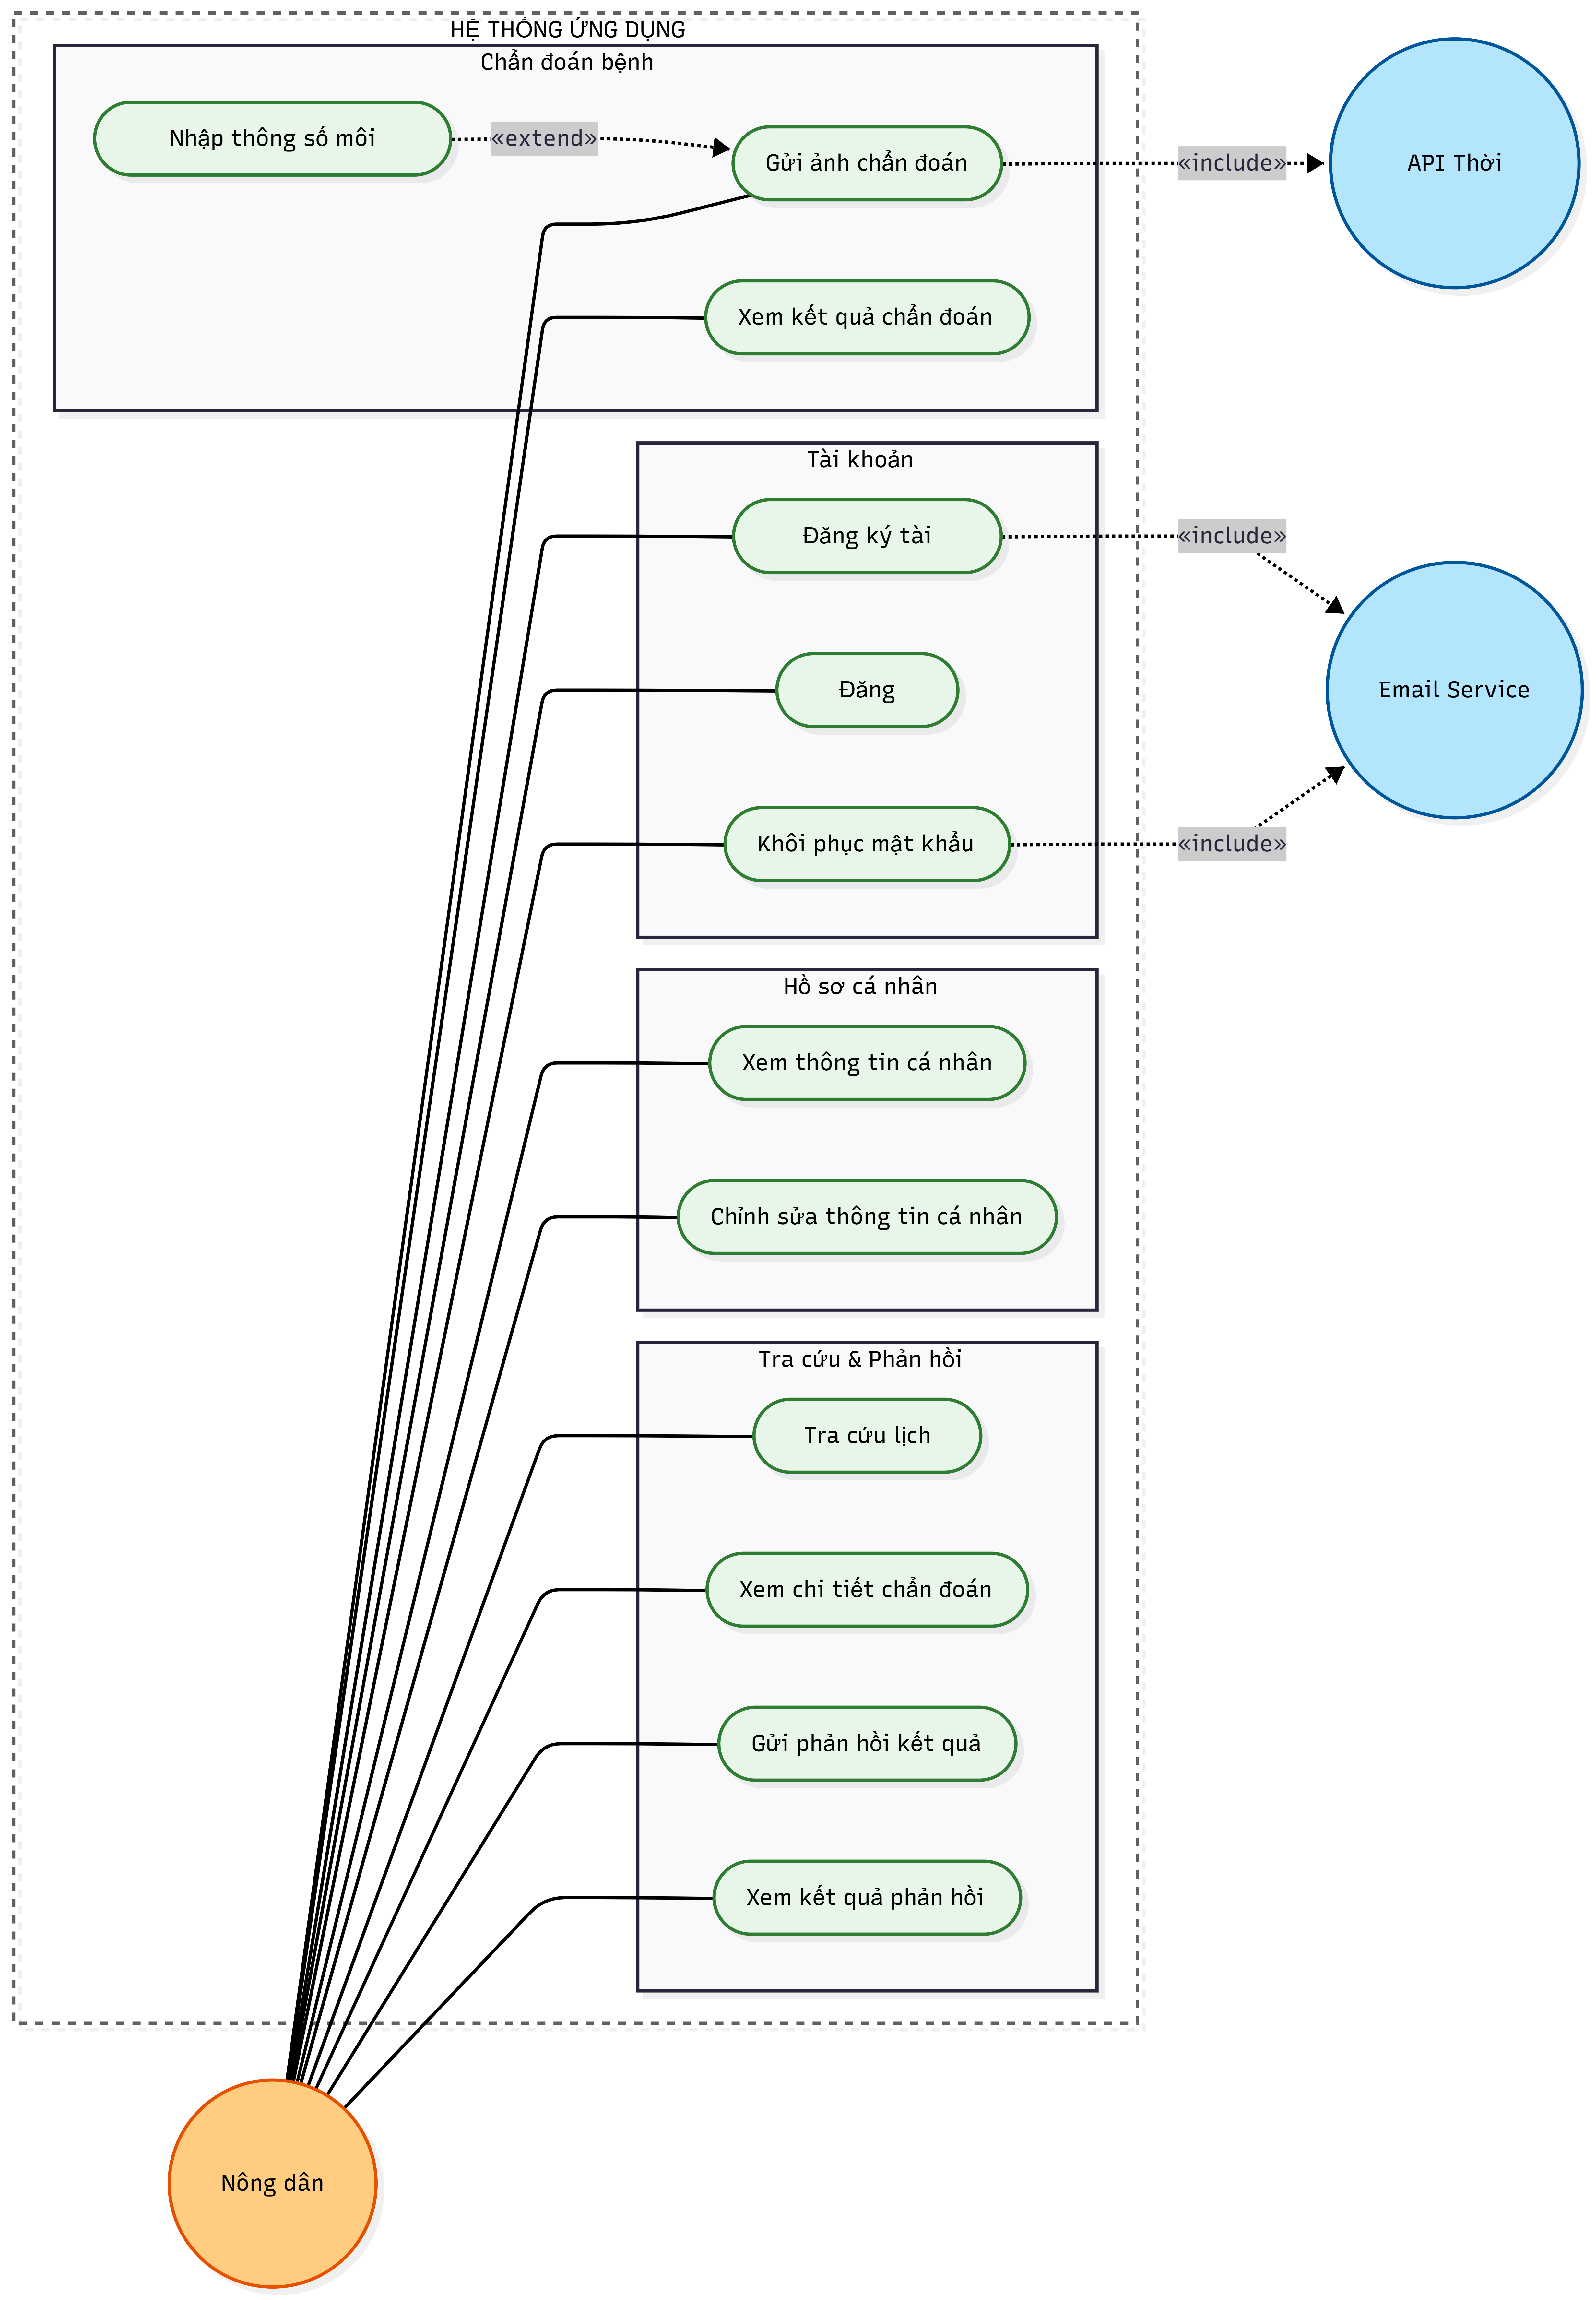
\includegraphics[width=\textwidth,height=0.85\textheight,keepaspectratio]{usecase-nongdan.png}
    \caption{Biểu đồ Use Case: Người dùng Nông dân}
    \label{fig:usecase-nongdan}
\end{figure}

\subsection{Biểu đồ Use Case --- Quản trị viên}

% Chèn ảnh Use Case Admin (xuất từ Mermaid/draw.io)
% \noindent\textit{[Chèn ảnh Use Case Quản trị viên tại đây]}
\begin{figure}[htbp]
    \centering
    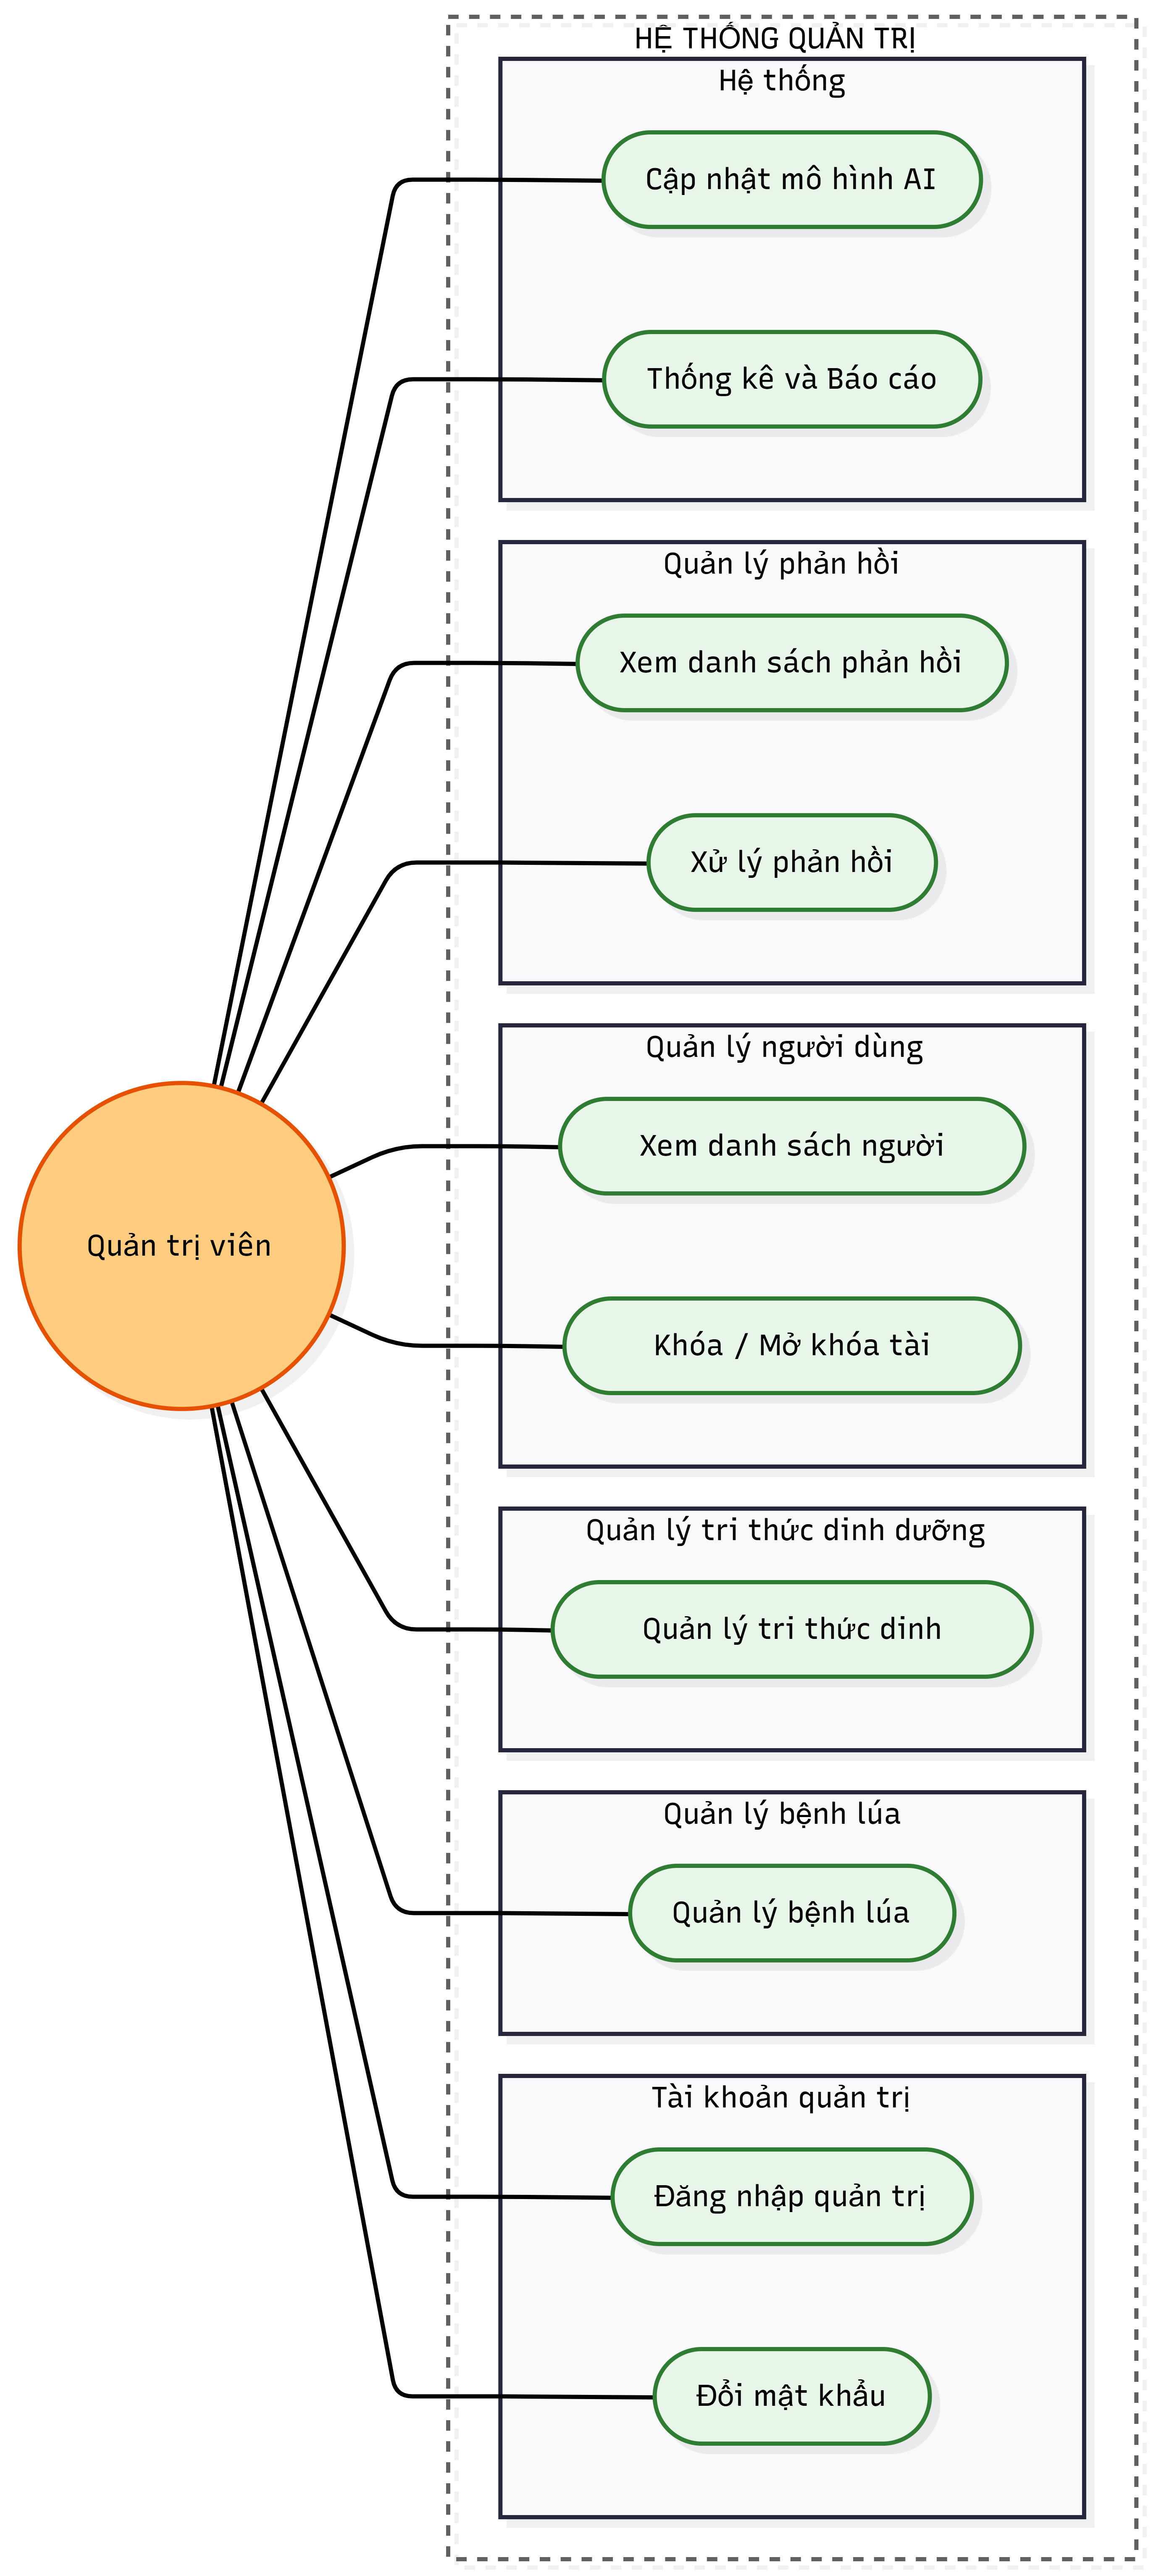
\includegraphics[width=\textwidth,height=0.85\textheight,keepaspectratio]{usecase-admin.png}
    \caption{Biểu đồ Use Case: Người dùng Quản trị viên}
    \label{fig:usecase-admin}
\end{figure}

\subsection{Bảng ký hiệu UML}

\begin{longtable}{|l|p{11cm}|}
    \hline
    \rowcolor{headerblue}
    \textbf{Ký hiệu}                       & \textbf{Ý nghĩa}                            \\
    \hline
    Hình người (stick figure)              & Actor --- tác nhân tương tác với hệ thống   \\
    \hline
    Hình elip                              & Use Case --- chức năng hệ thống             \\
    \hline
    Hình chữ nhật bao quanh                & System Boundary --- ranh giới hệ thống      \\
    \hline
    Đường liền                             & Association --- actor sử dụng use case      \\
    \hline
    Mũi tên đứt nét + \texttt{<<include>>} & Use case bắt buộc gọi đến use case khác     \\
    \hline
    Mũi tên đứt nét + \texttt{<<extend>>}  & Use case mở rộng (tùy chọn, không bắt buộc) \\
    \hline
\end{longtable}

\hrulefill

% ============================================================
\section{Biểu đồ tuần tự (Sequence Diagrams)}

\subsection{SD-01: Đăng ký tài khoản (có xác thực email)}
% \noindent\textit{[Chèn ảnh SD-01 tại đây]}
\begin{figure}[htbp]
    \centering
    \includegraphics[width=\textwidth,height=0.85\textheight,keepaspectratio]{sd-01-register.png}
    \caption{Biểu đồ tuần tự: Đăng ký tài khoản}
    \label{fig:sd-01}
\end{figure}

\subsection{SD-02: Đăng nhập hệ thống}
% \noindent\textit{[Chèn ảnh SD-02 tại đây]}
\begin{figure}[htbp]
    \centering
    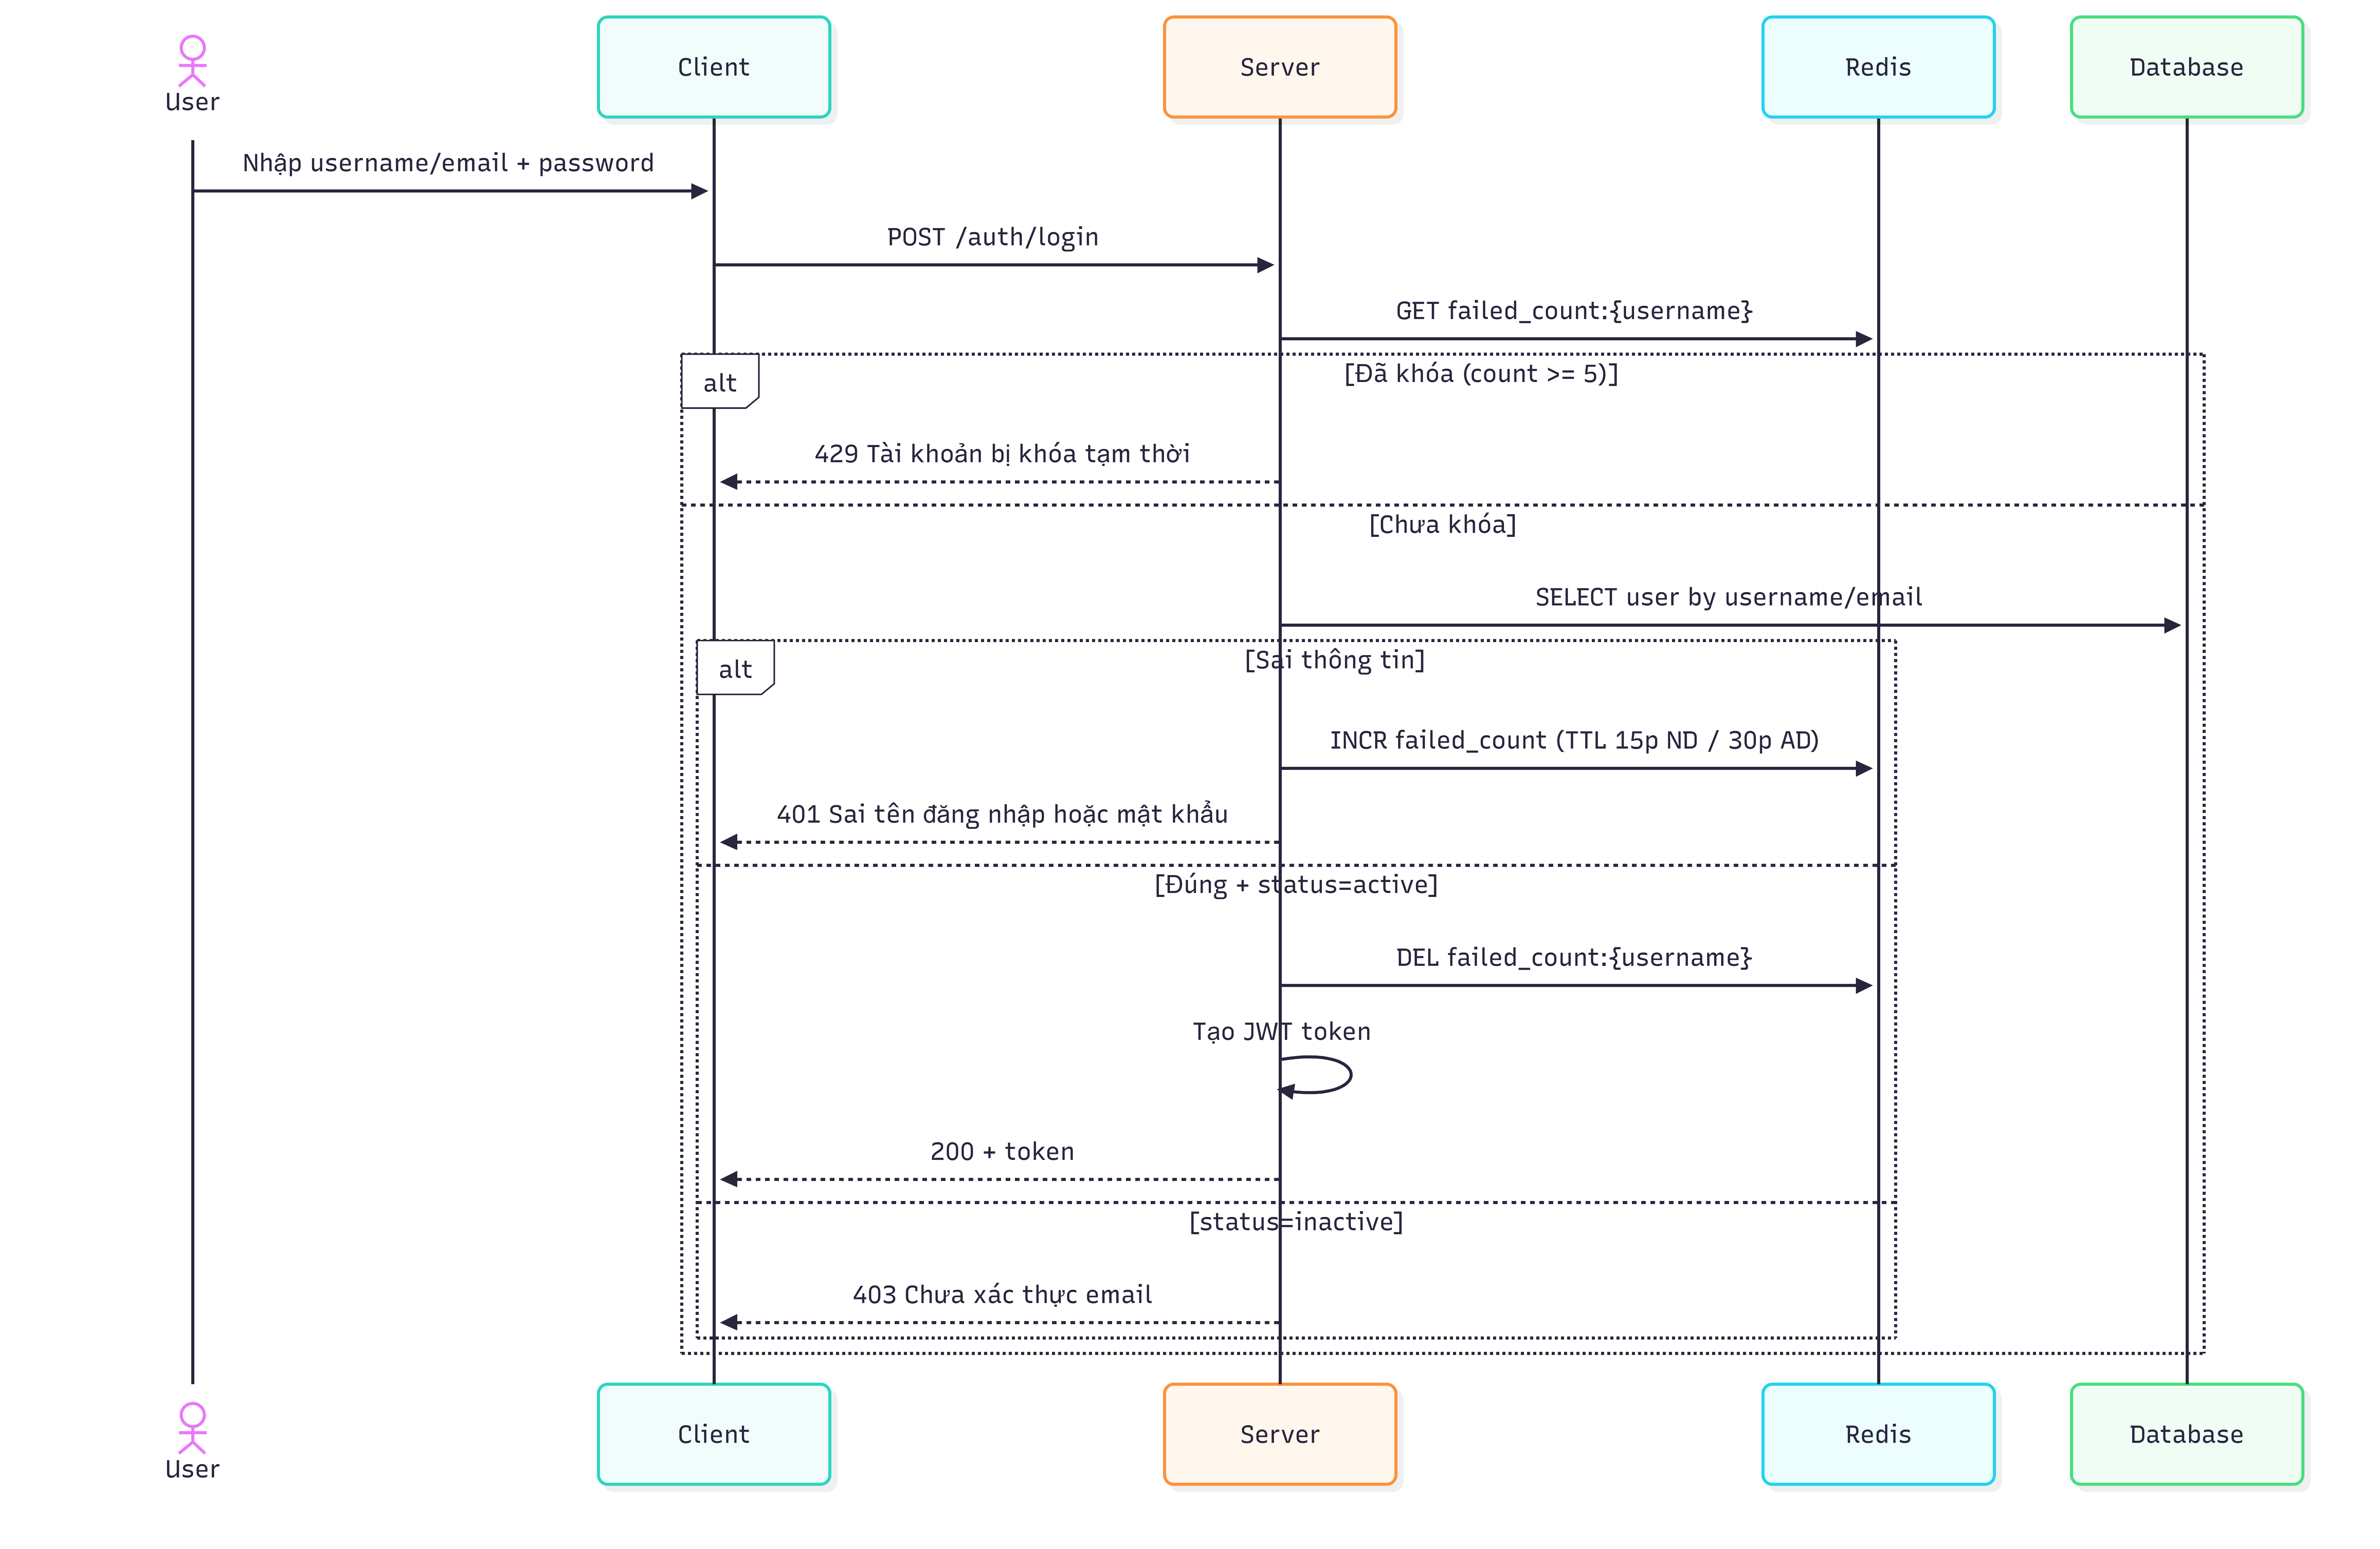
\includegraphics[width=\textwidth,height=0.85\textheight,keepaspectratio]{sd-02-login.png}
    \caption{Biểu đồ tuần tự: Đăng nhập hệ thống}
    \label{fig:sd-02}
\end{figure}

\subsection{SD-03: Khôi phục mật khẩu}
% \noindent\textit{[Chèn ảnh SD-03 tại đây]}
\begin{figure}[htbp]
    \centering
    \includegraphics[width=\textwidth,height=0.85\textheight,keepaspectratio]{sd-03-forgot-password.png}
    \caption{Biểu đồ tuần tự: Khôi phục mật khẩu}
    \label{fig:sd-03}
\end{figure}

\subsection{SD-04: Xem \& Chỉnh sửa hồ sơ cá nhân}
% \noindent\textit{[Chèn ảnh SD-04 tại đây]}
\begin{figure}[htbp]
    \centering
    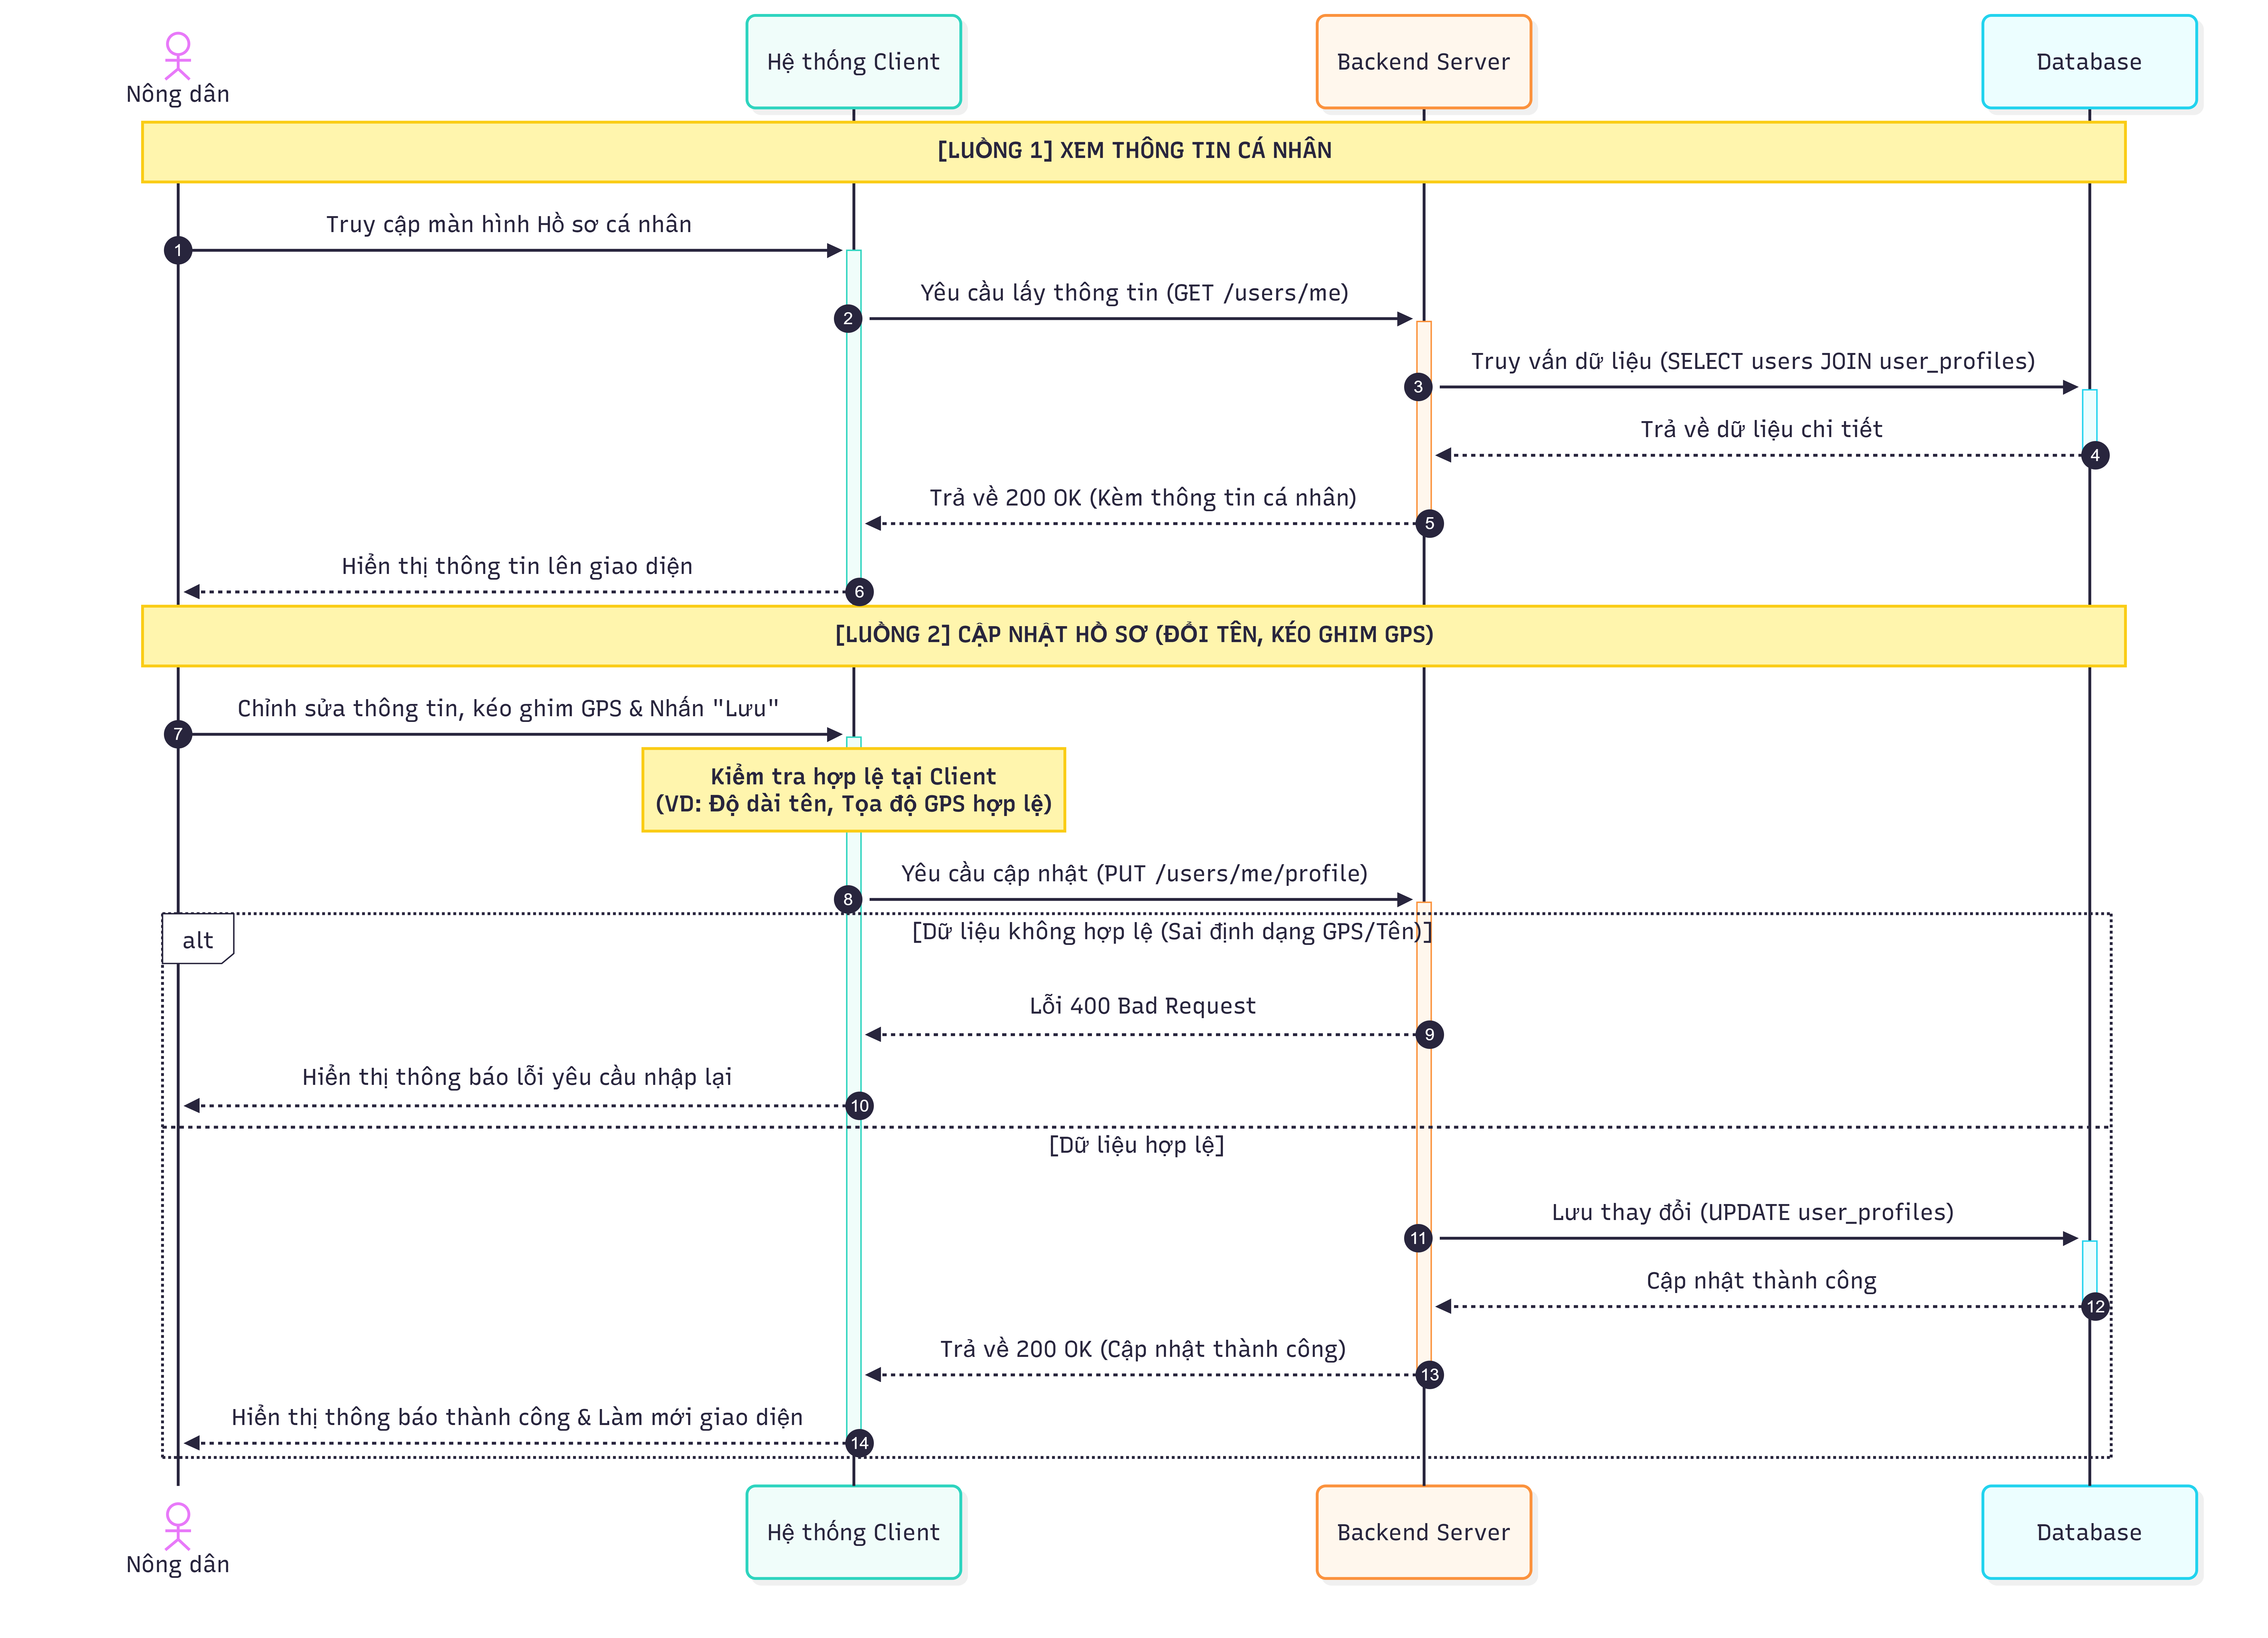
\includegraphics[width=\textwidth,height=0.85\textheight,keepaspectratio]{sd-04-profile.png}
    \caption{Biểu đồ tuần tự: Xem và chỉnh sửa hồ sơ cá nhân}
    \label{fig:sd-04}
\end{figure}

\subsection{SD-05: Gửi ảnh chẩn đoán (Core Flow)}
% \noindent\textit{[Chèn ảnh SD-05 tại đây]}
\begin{figure}[htbp]
    \centering
    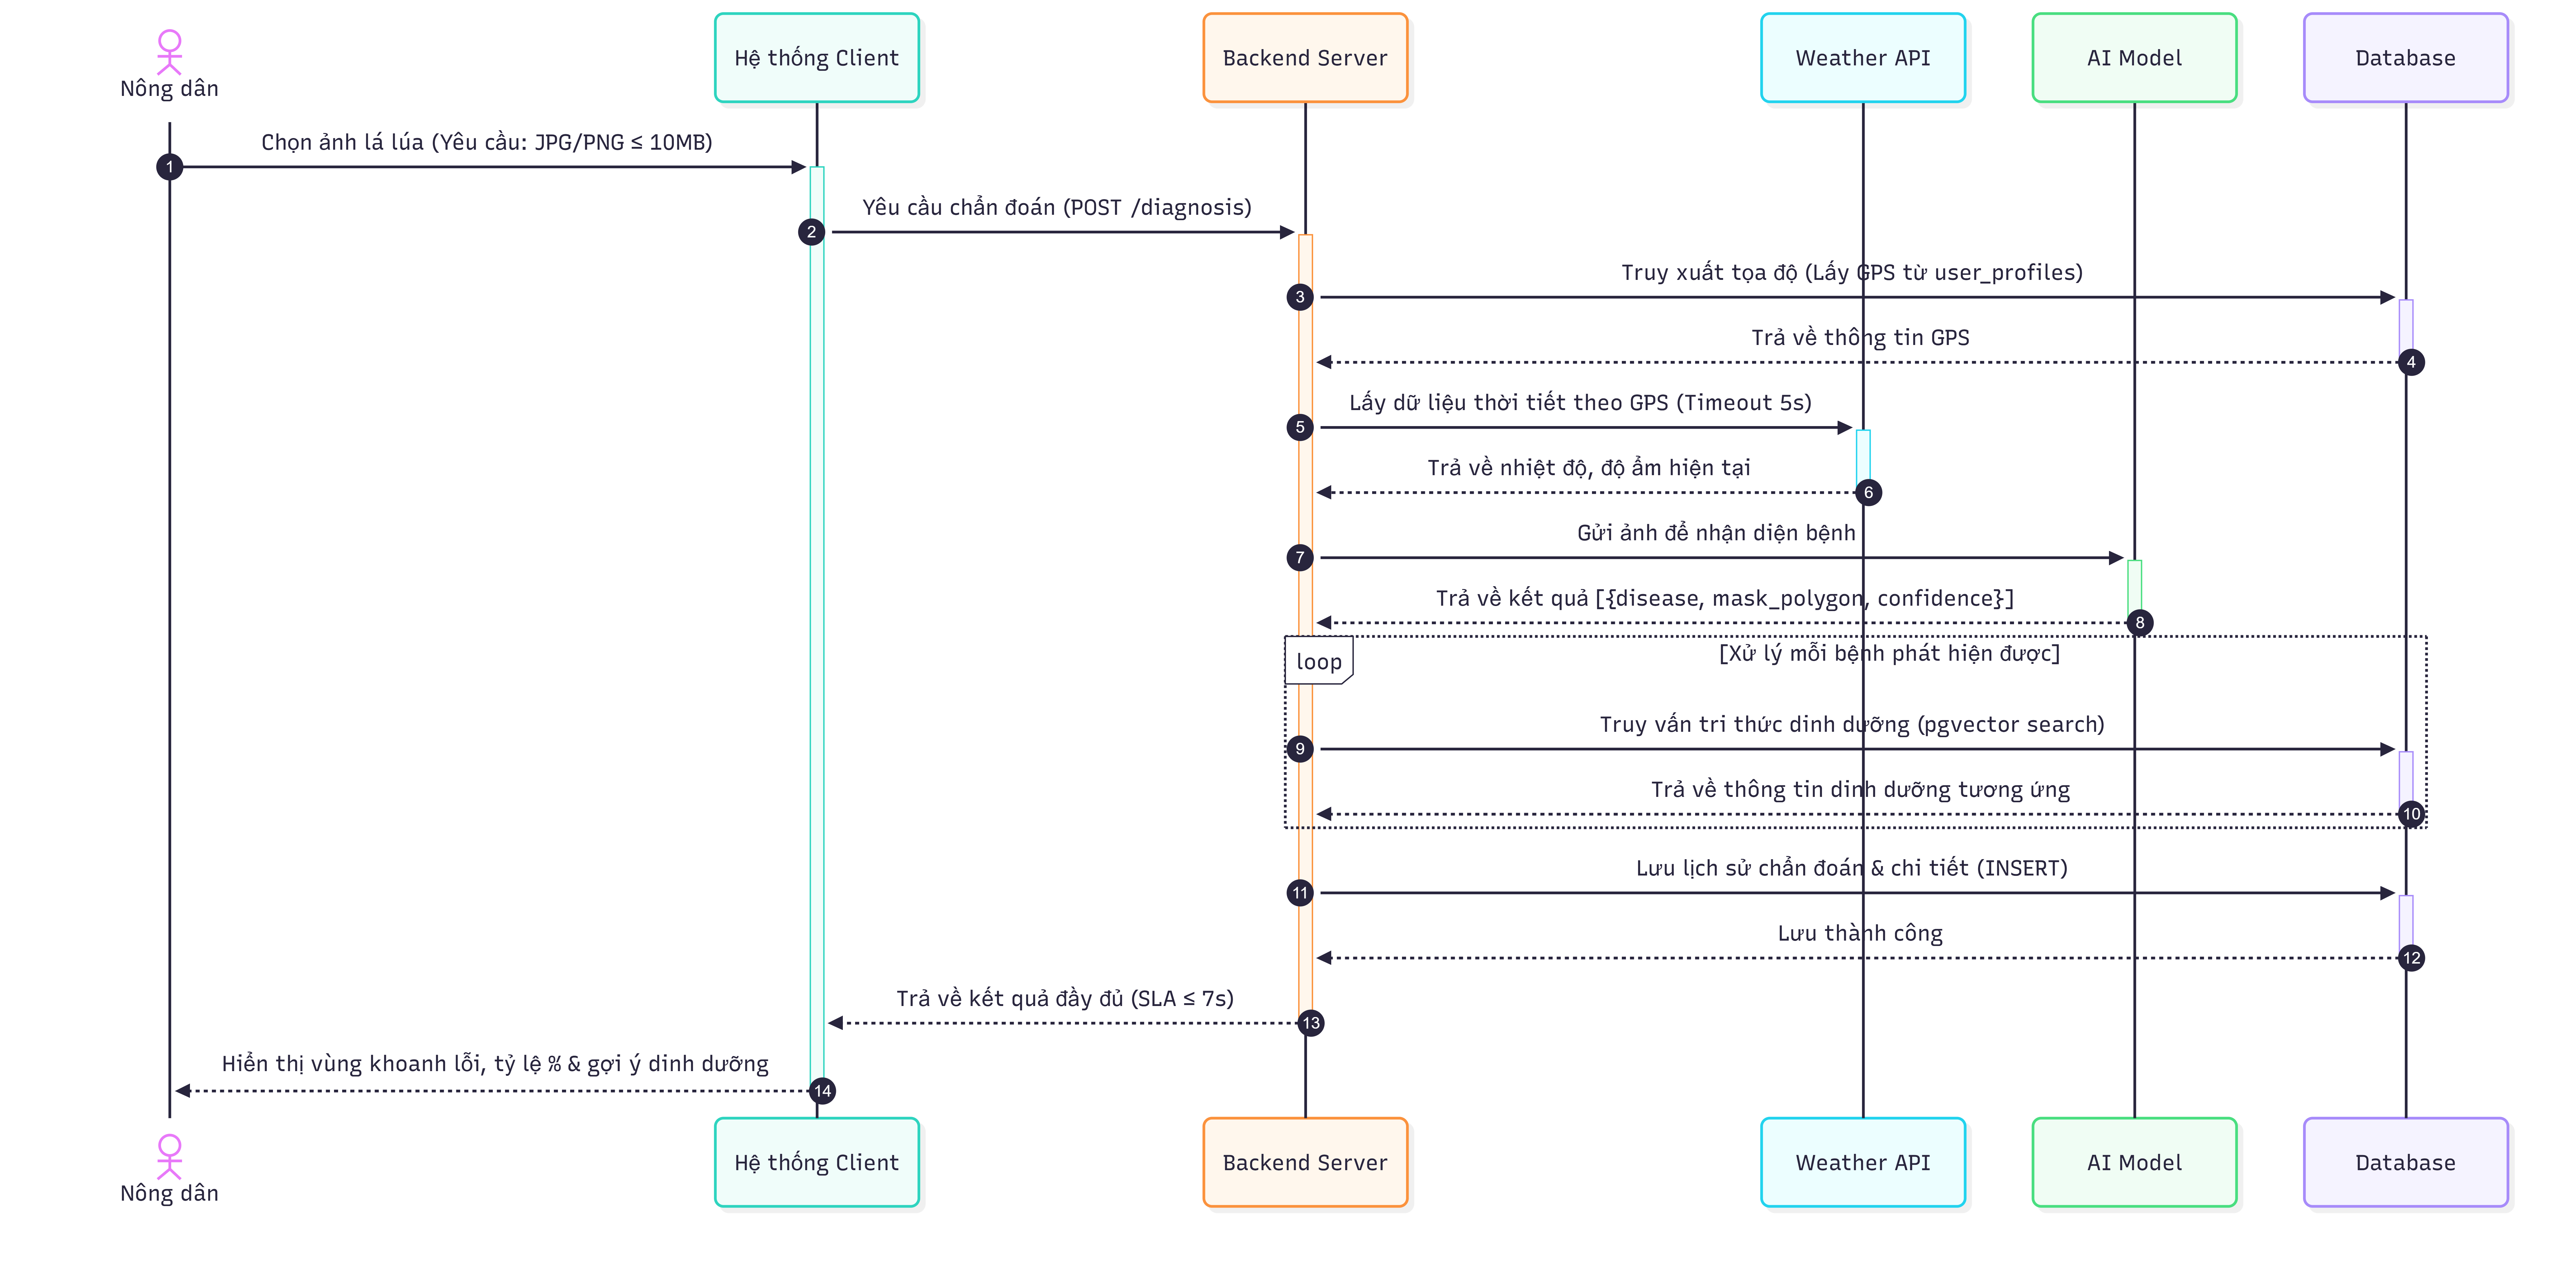
\includegraphics[width=\textwidth,height=0.85\textheight,keepaspectratio]{sd-05-diagnosis.png}
    \caption{Biểu đồ tuần tự: Gửi ảnh chẩn đoán}
    \label{fig:sd-05}
\end{figure}

\subsection{SD-06: Nhập thông số môi trường bổ sung}
% \noindent\textit{[Chèn ảnh SD-06 tại đây]}
\begin{figure}[htbp]
    \centering
    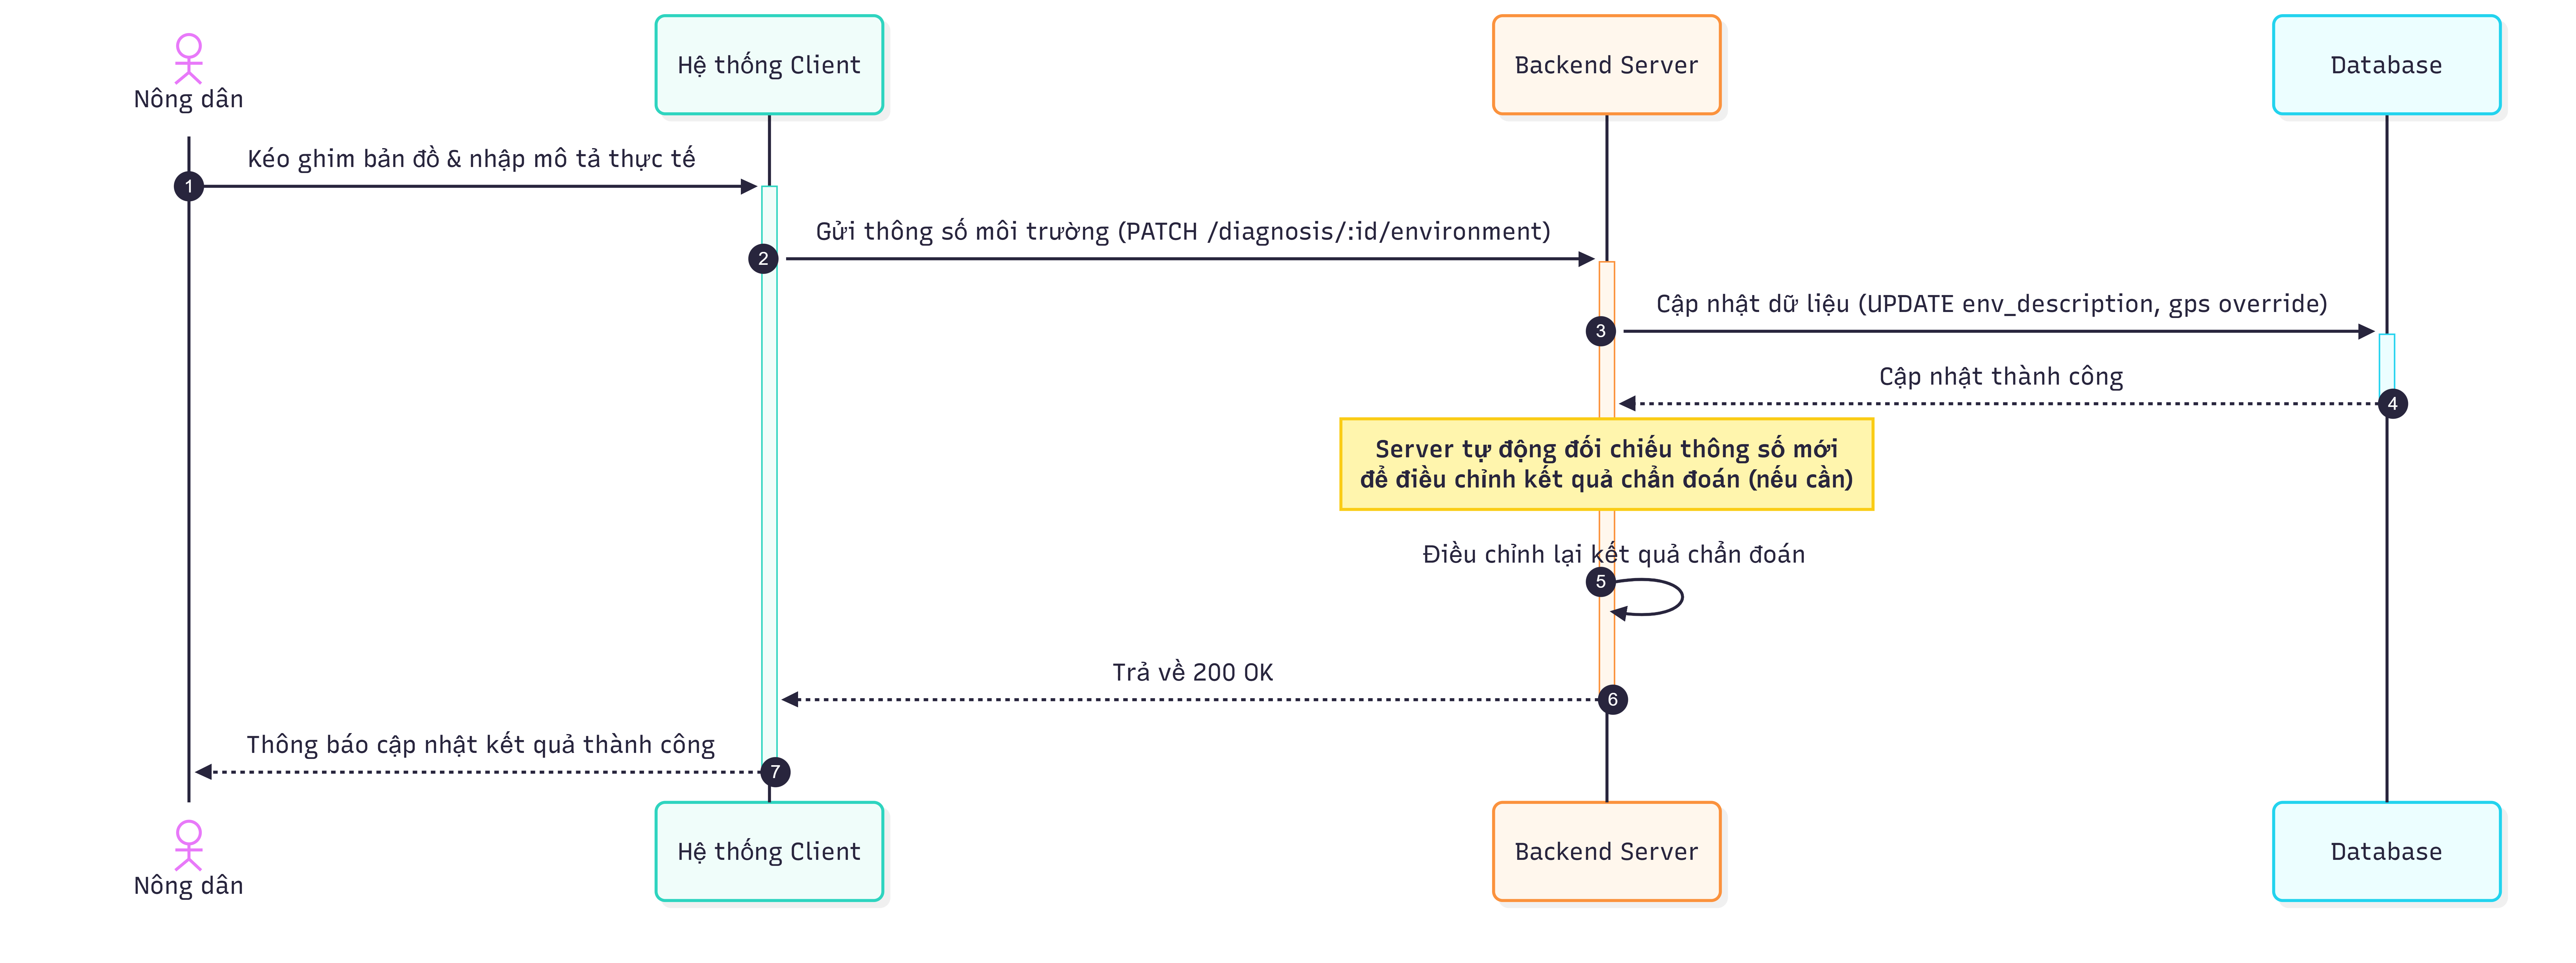
\includegraphics[width=\textwidth,height=0.85\textheight,keepaspectratio]{sd-06-environment.png}
    \caption{Biểu đồ tuần tự: Nhập thông số môi trường bổ sung}
    \label{fig:sd-06}
\end{figure}

\subsection{SD-07: Tra cứu lịch sử \& Xem chi tiết}
% \noindent\textit{[Chèn ảnh SD-07 tại đây]}
\begin{figure}[htbp]
    \centering
    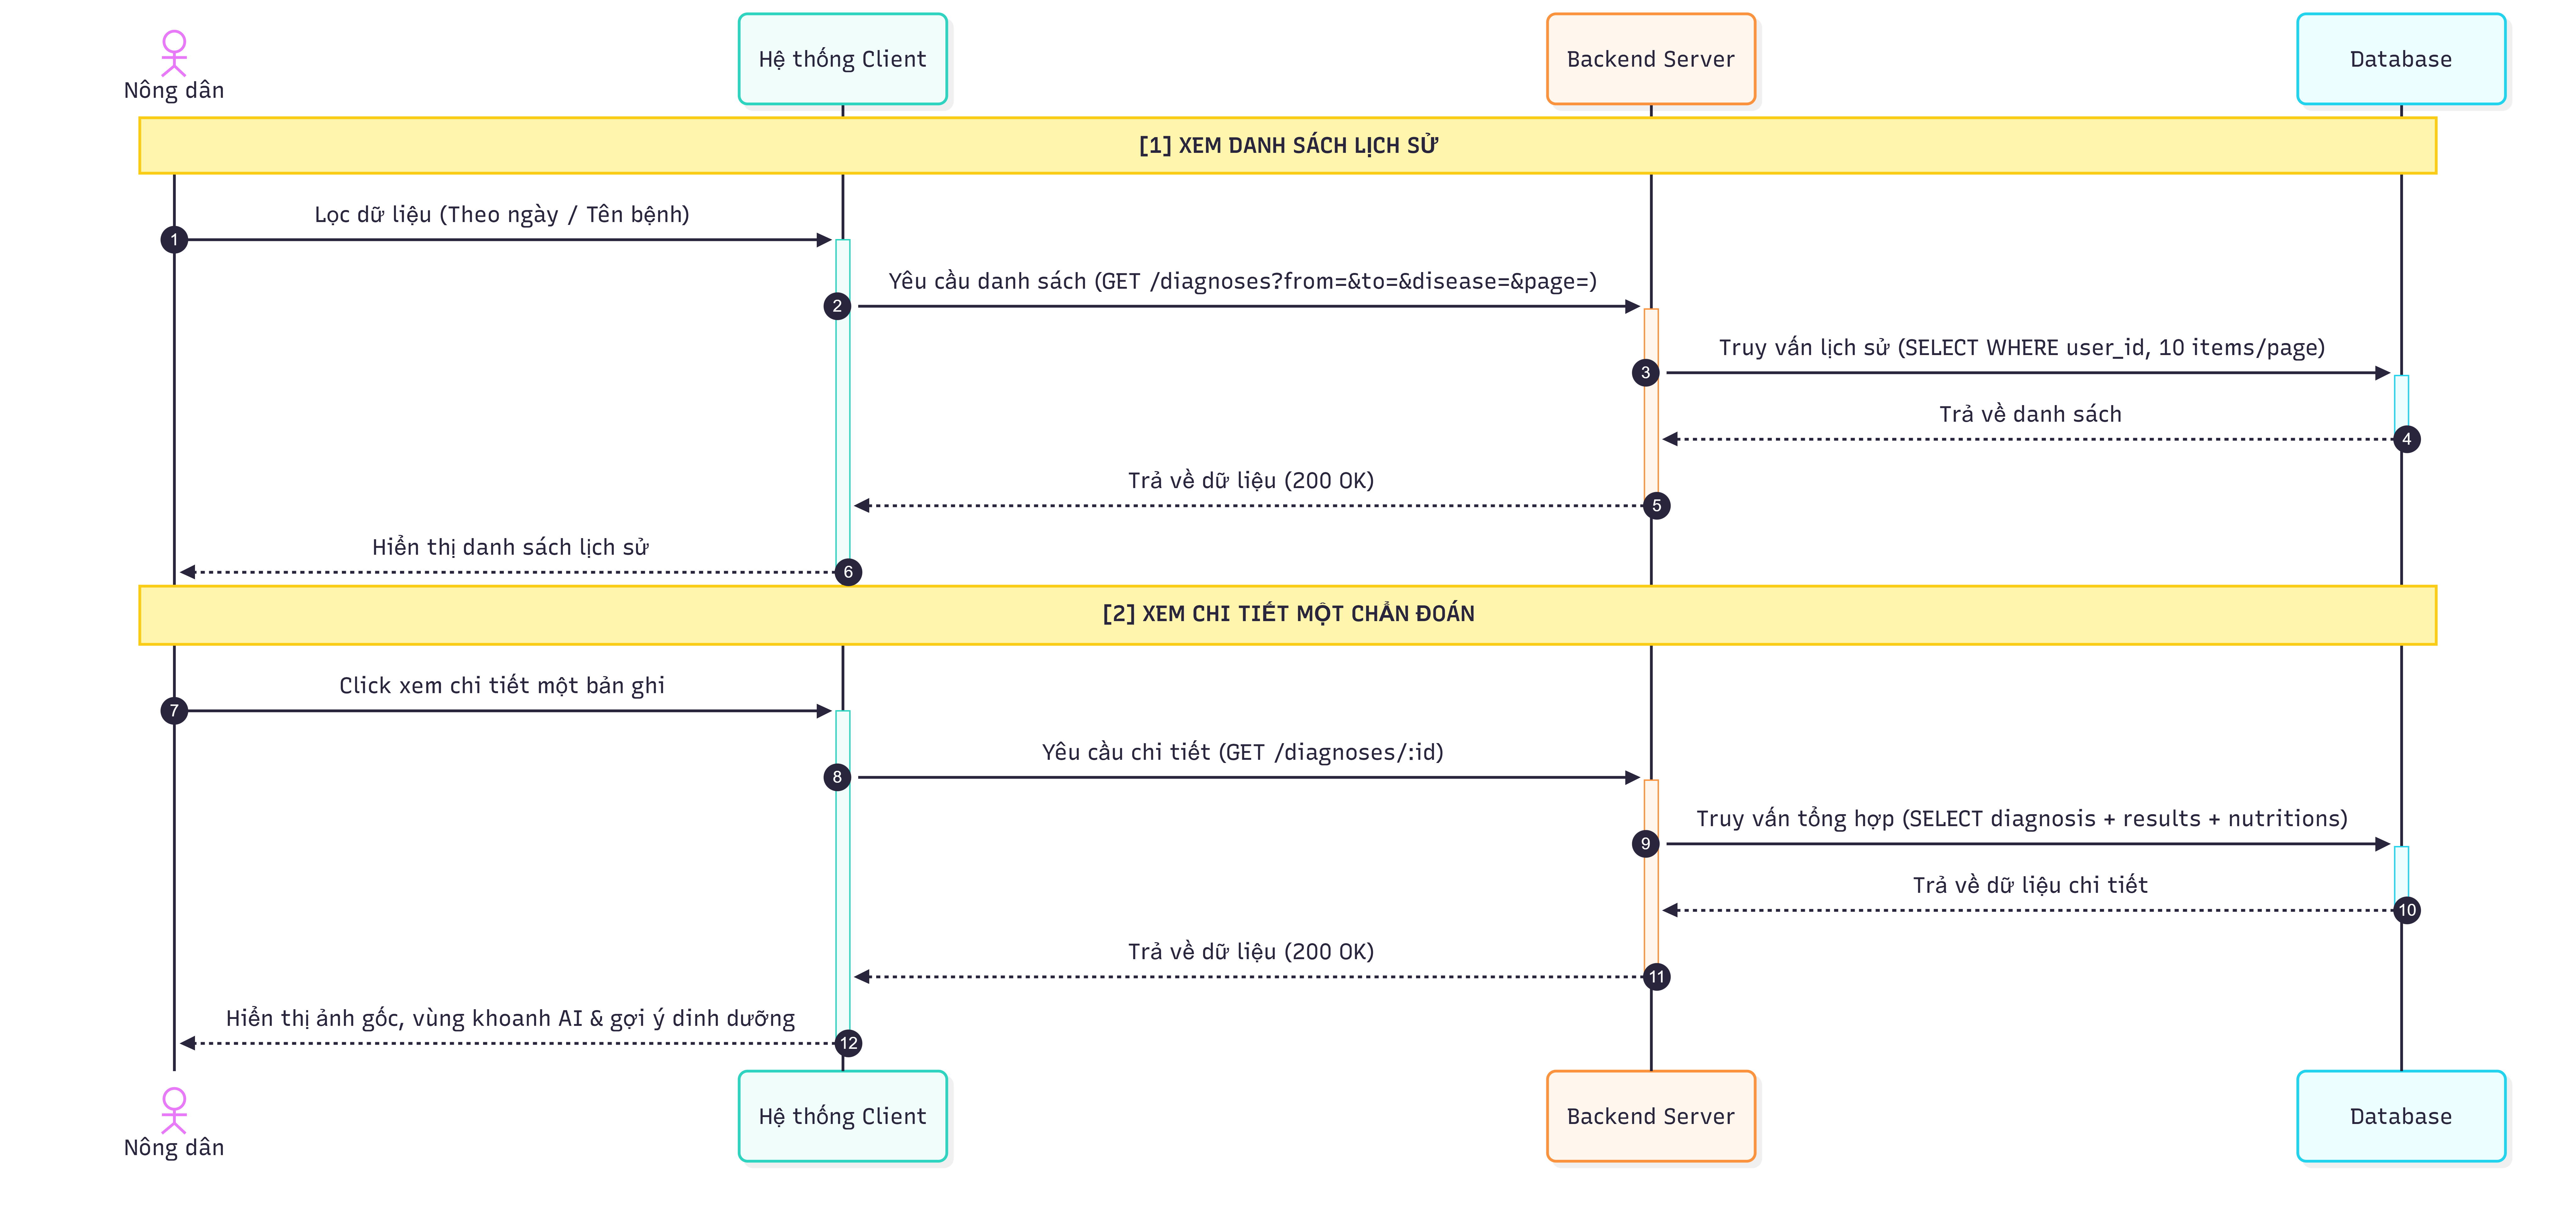
\includegraphics[width=\textwidth,height=0.85\textheight,keepaspectratio]{sd-07-history.png}
    \caption{Biểu đồ tuần tự: Tra cứu lịch sử và xem chi tiết}
    \label{fig:sd-07}
\end{figure}

\subsection{SD-08: Gửi phản hồi kết quả \& SD-09: Xem kết quả xử lý phản hồi}
% \noindent\textit{[Chèn ảnh SD-08, SD-09 tại đây]}
\begin{figure}[htbp]
    \centering
    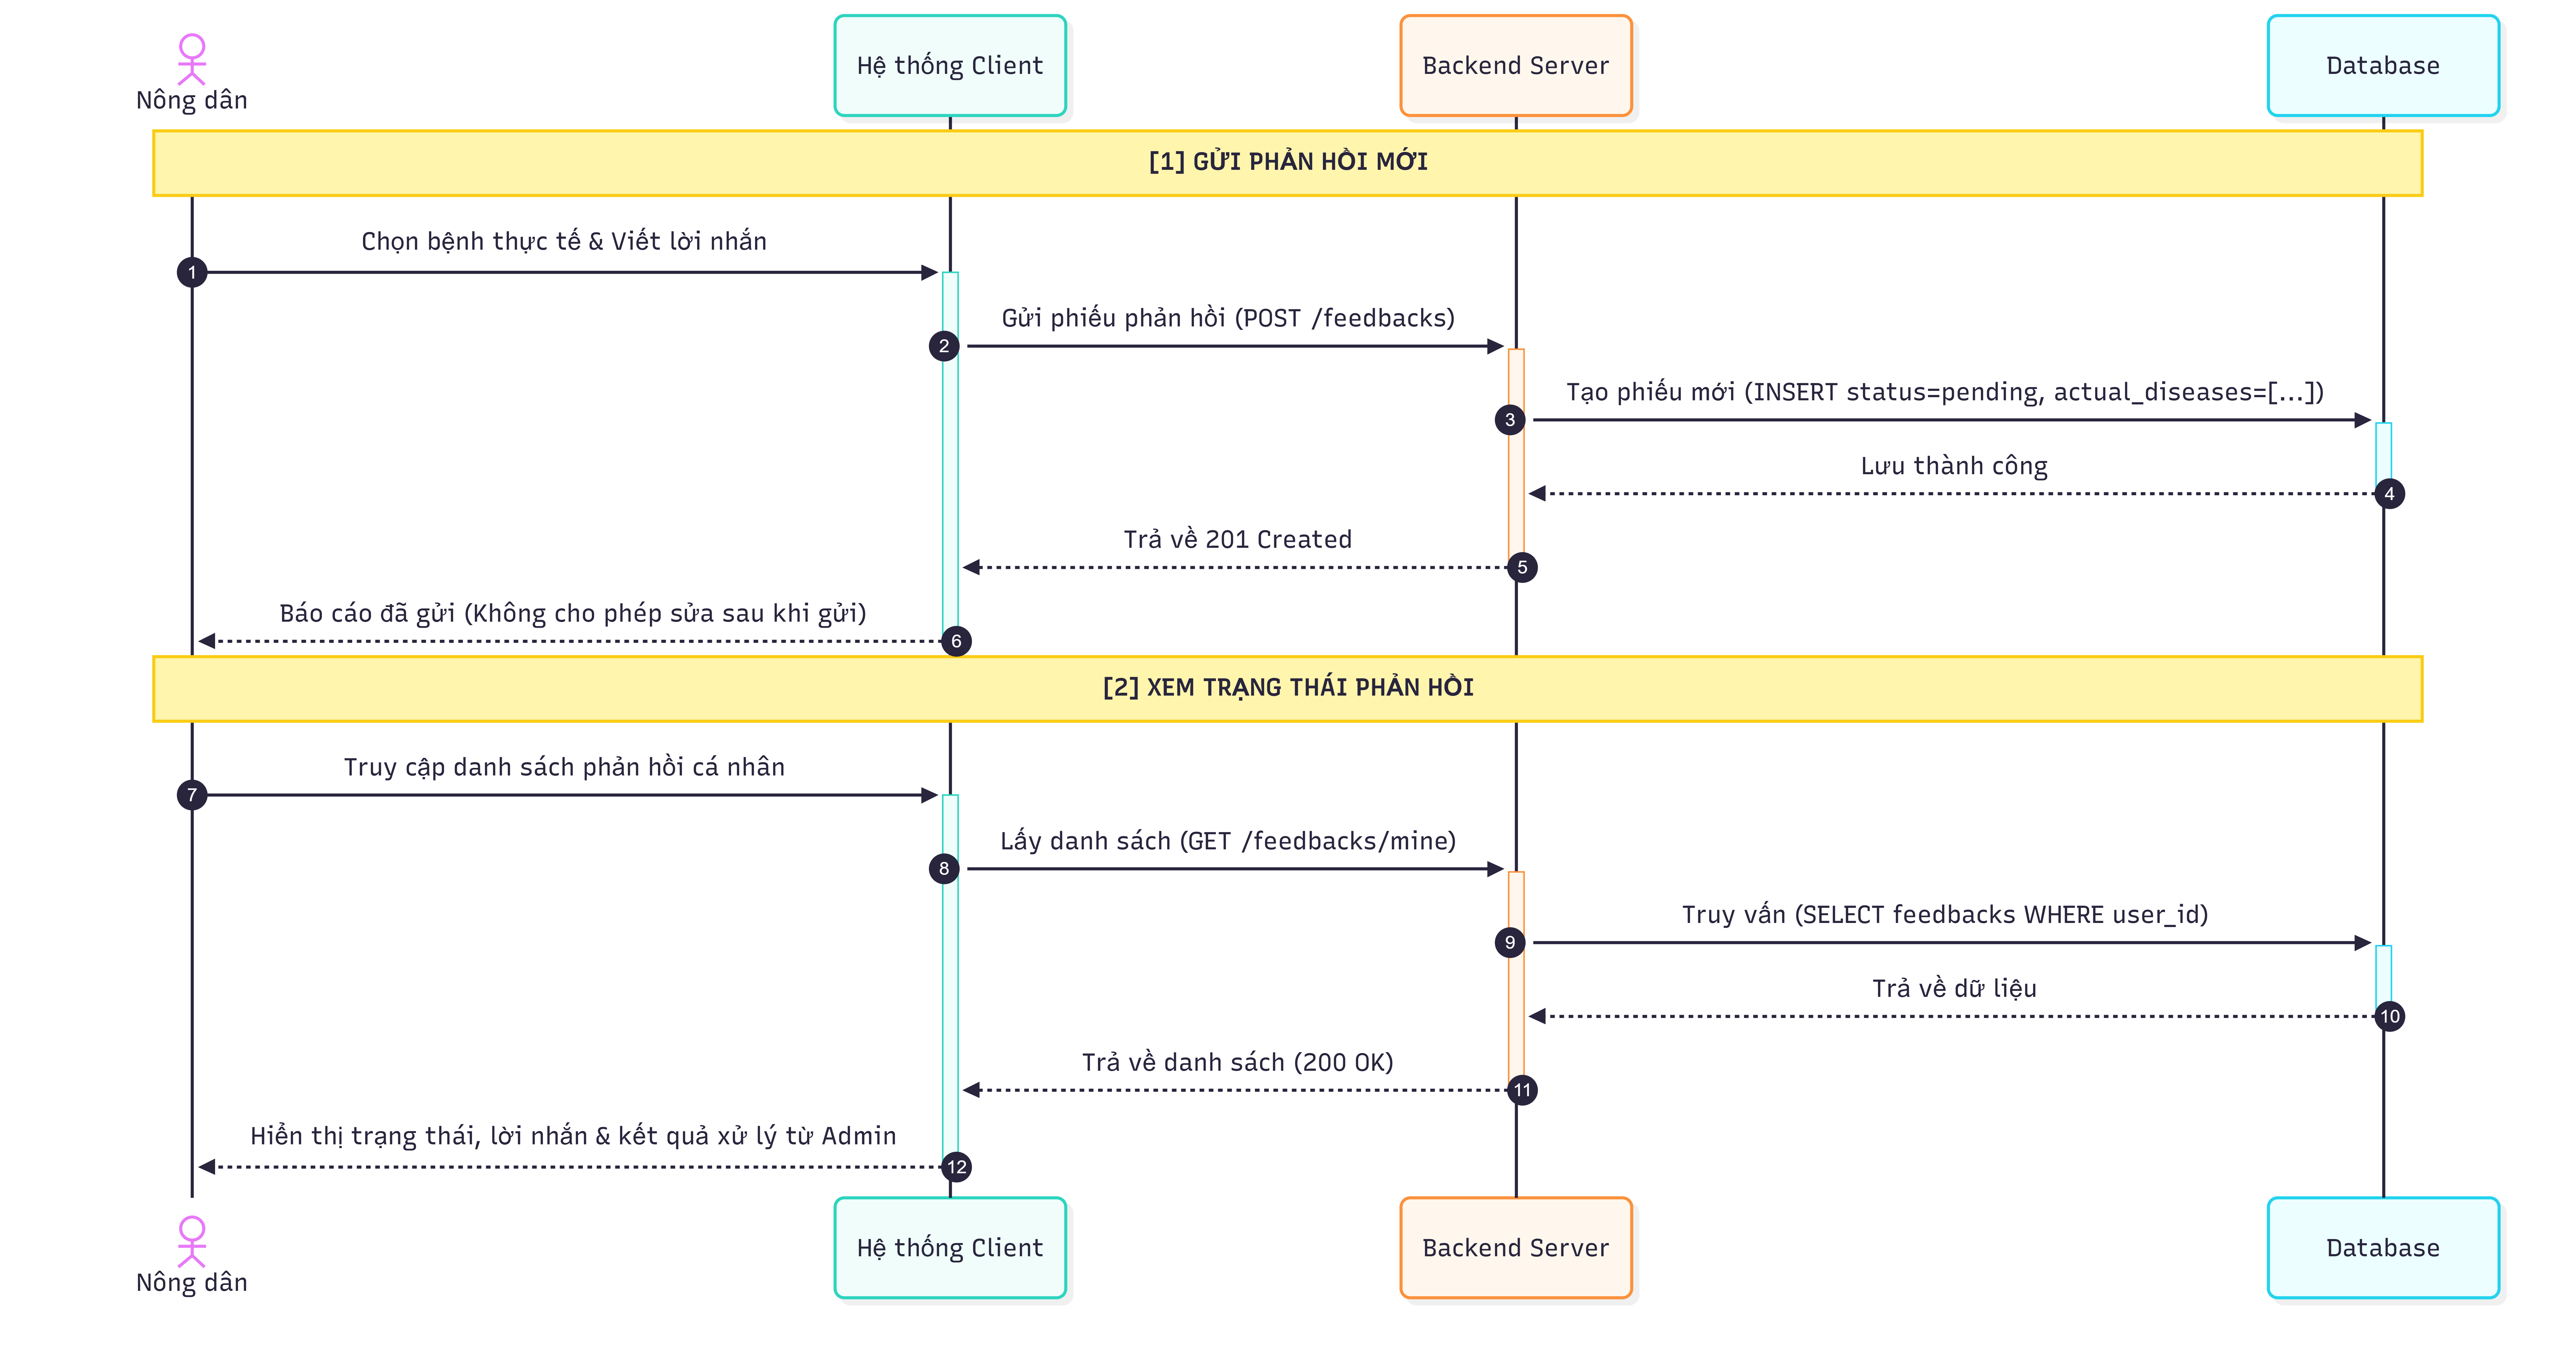
\includegraphics[width=\textwidth,height=0.85\textheight,keepaspectratio]{sd-0809-feedback.png}
    \caption{Biểu đồ tuần tự: Gửi phản hồi và xem kết quả xử lý}
    \label{fig:sd-0809}
\end{figure}

\subsection{SD-10: Quản lý bệnh lúa (CRUD)}
% \noindent\textit{[Chèn ảnh SD-10 tại đây]}
\begin{figure}[htbp]
    \centering
    \includegraphics[width=\textwidth,height=0.85\textheight,keepaspectratio]{sd-10-disease-crud.png}
    \caption{Biểu đồ tuần tự: Quản lý bệnh lúa (CRUD)}
    \label{fig:sd-10}
\end{figure}

\subsection{SD-11: Quản lý tri thức dinh dưỡng}
% \noindent\textit{[Chèn ảnh SD-11 tại đây]}
\begin{figure}[htbp]
    \centering
    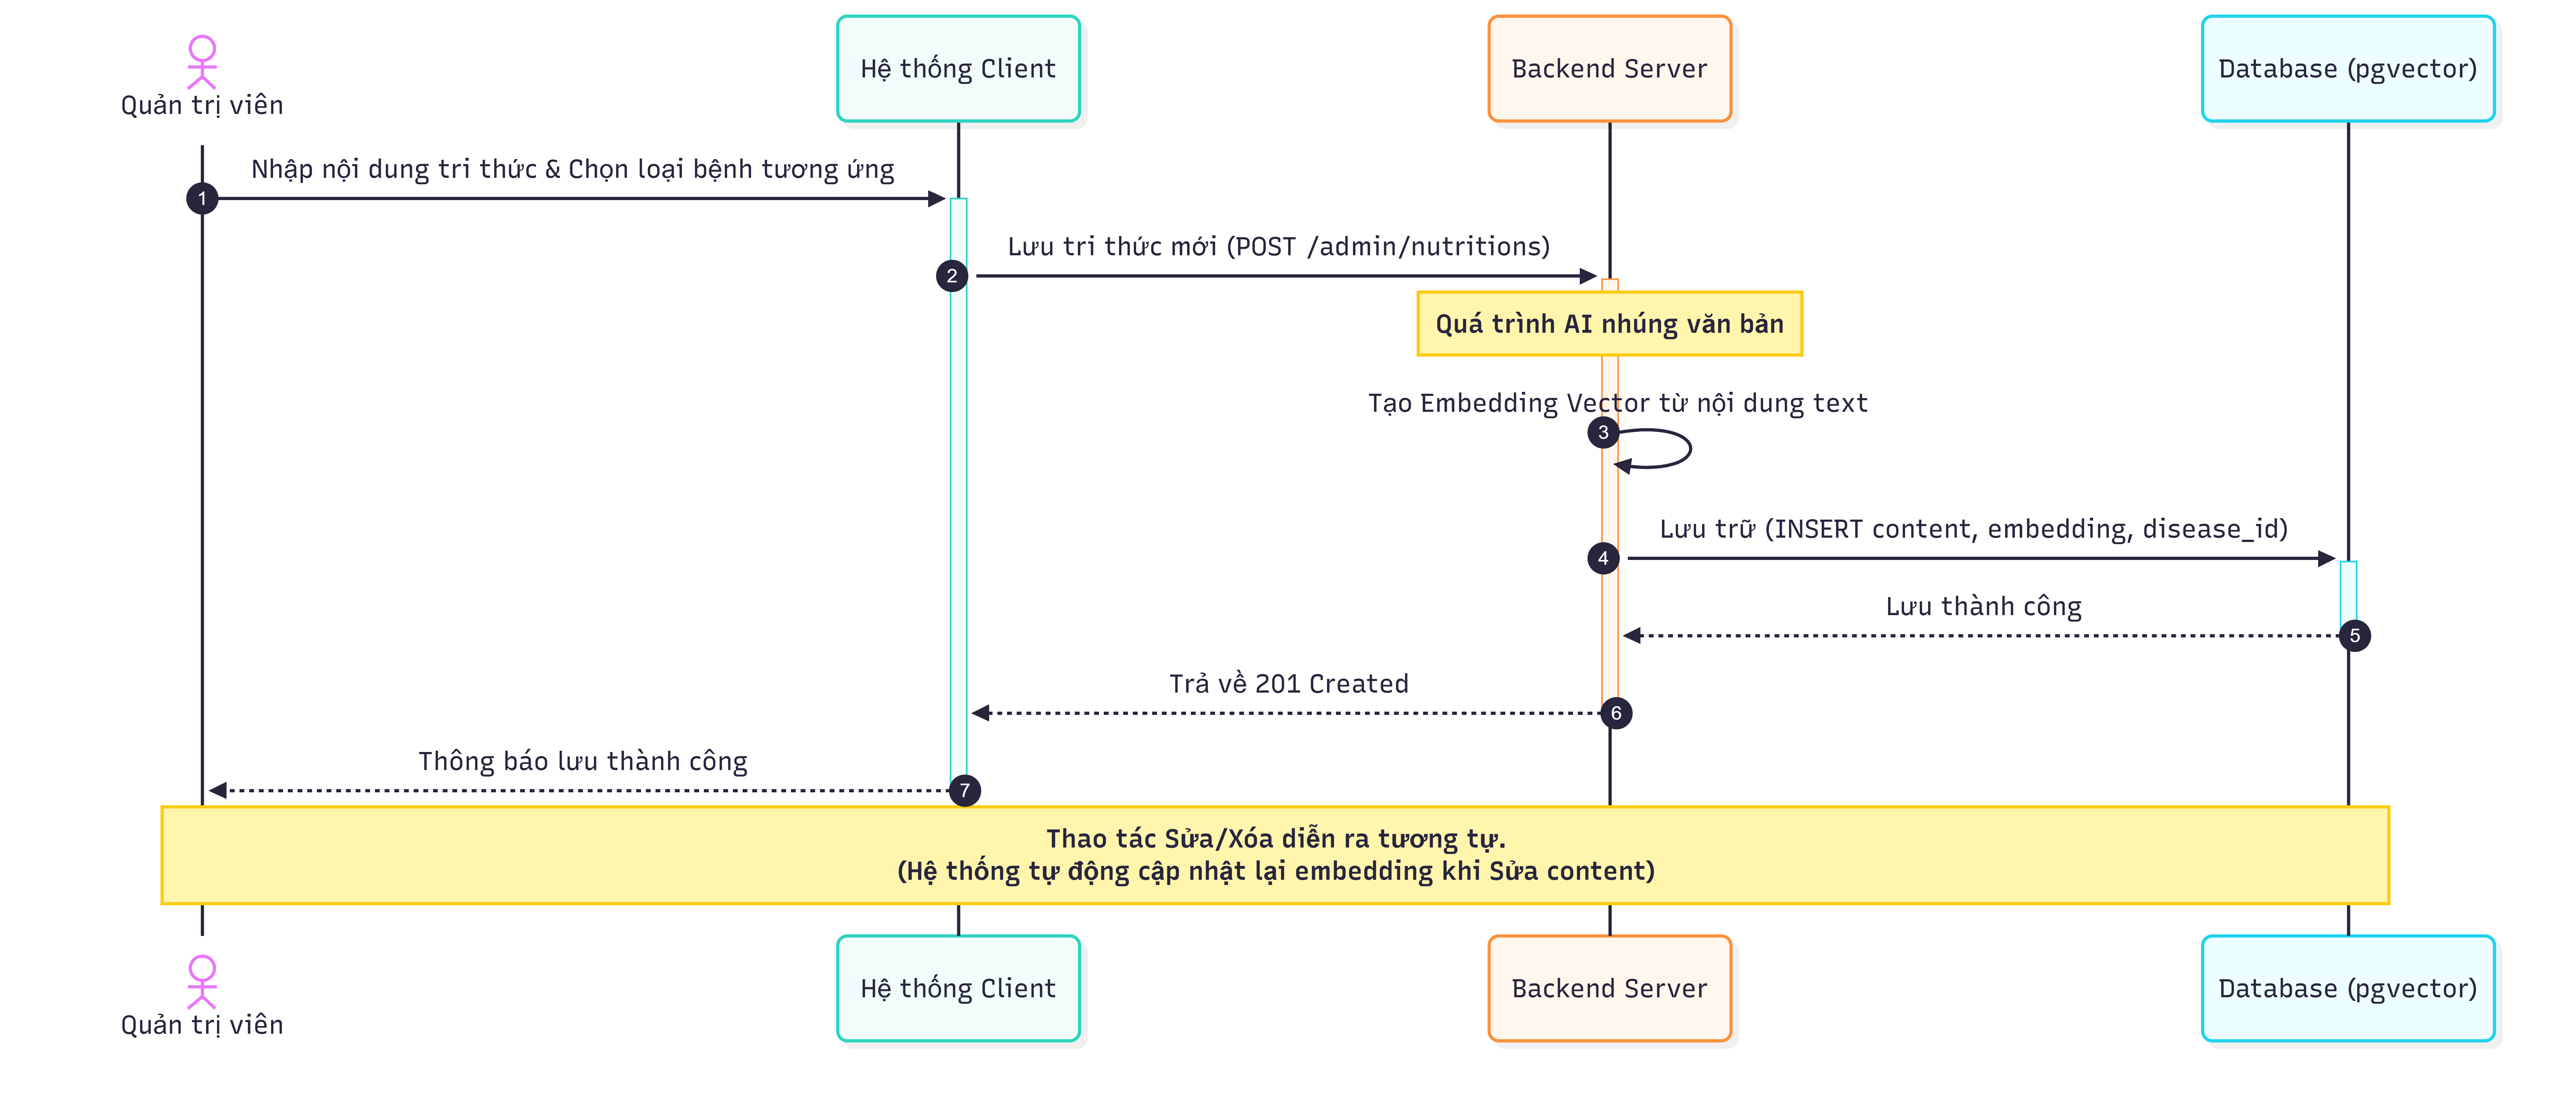
\includegraphics[width=\textwidth,height=0.85\textheight,keepaspectratio]{sd-11-nutrition.png}
    \caption{Biểu đồ tuần tự: Quản lý tri thức dinh dưỡng}
    \label{fig:sd-11}
\end{figure}

\subsection{SD-12: Quản lý người dùng}
% \noindent\textit{[Chèn ảnh SD-12 tại đây]}
\begin{figure}[htbp]
    \centering
    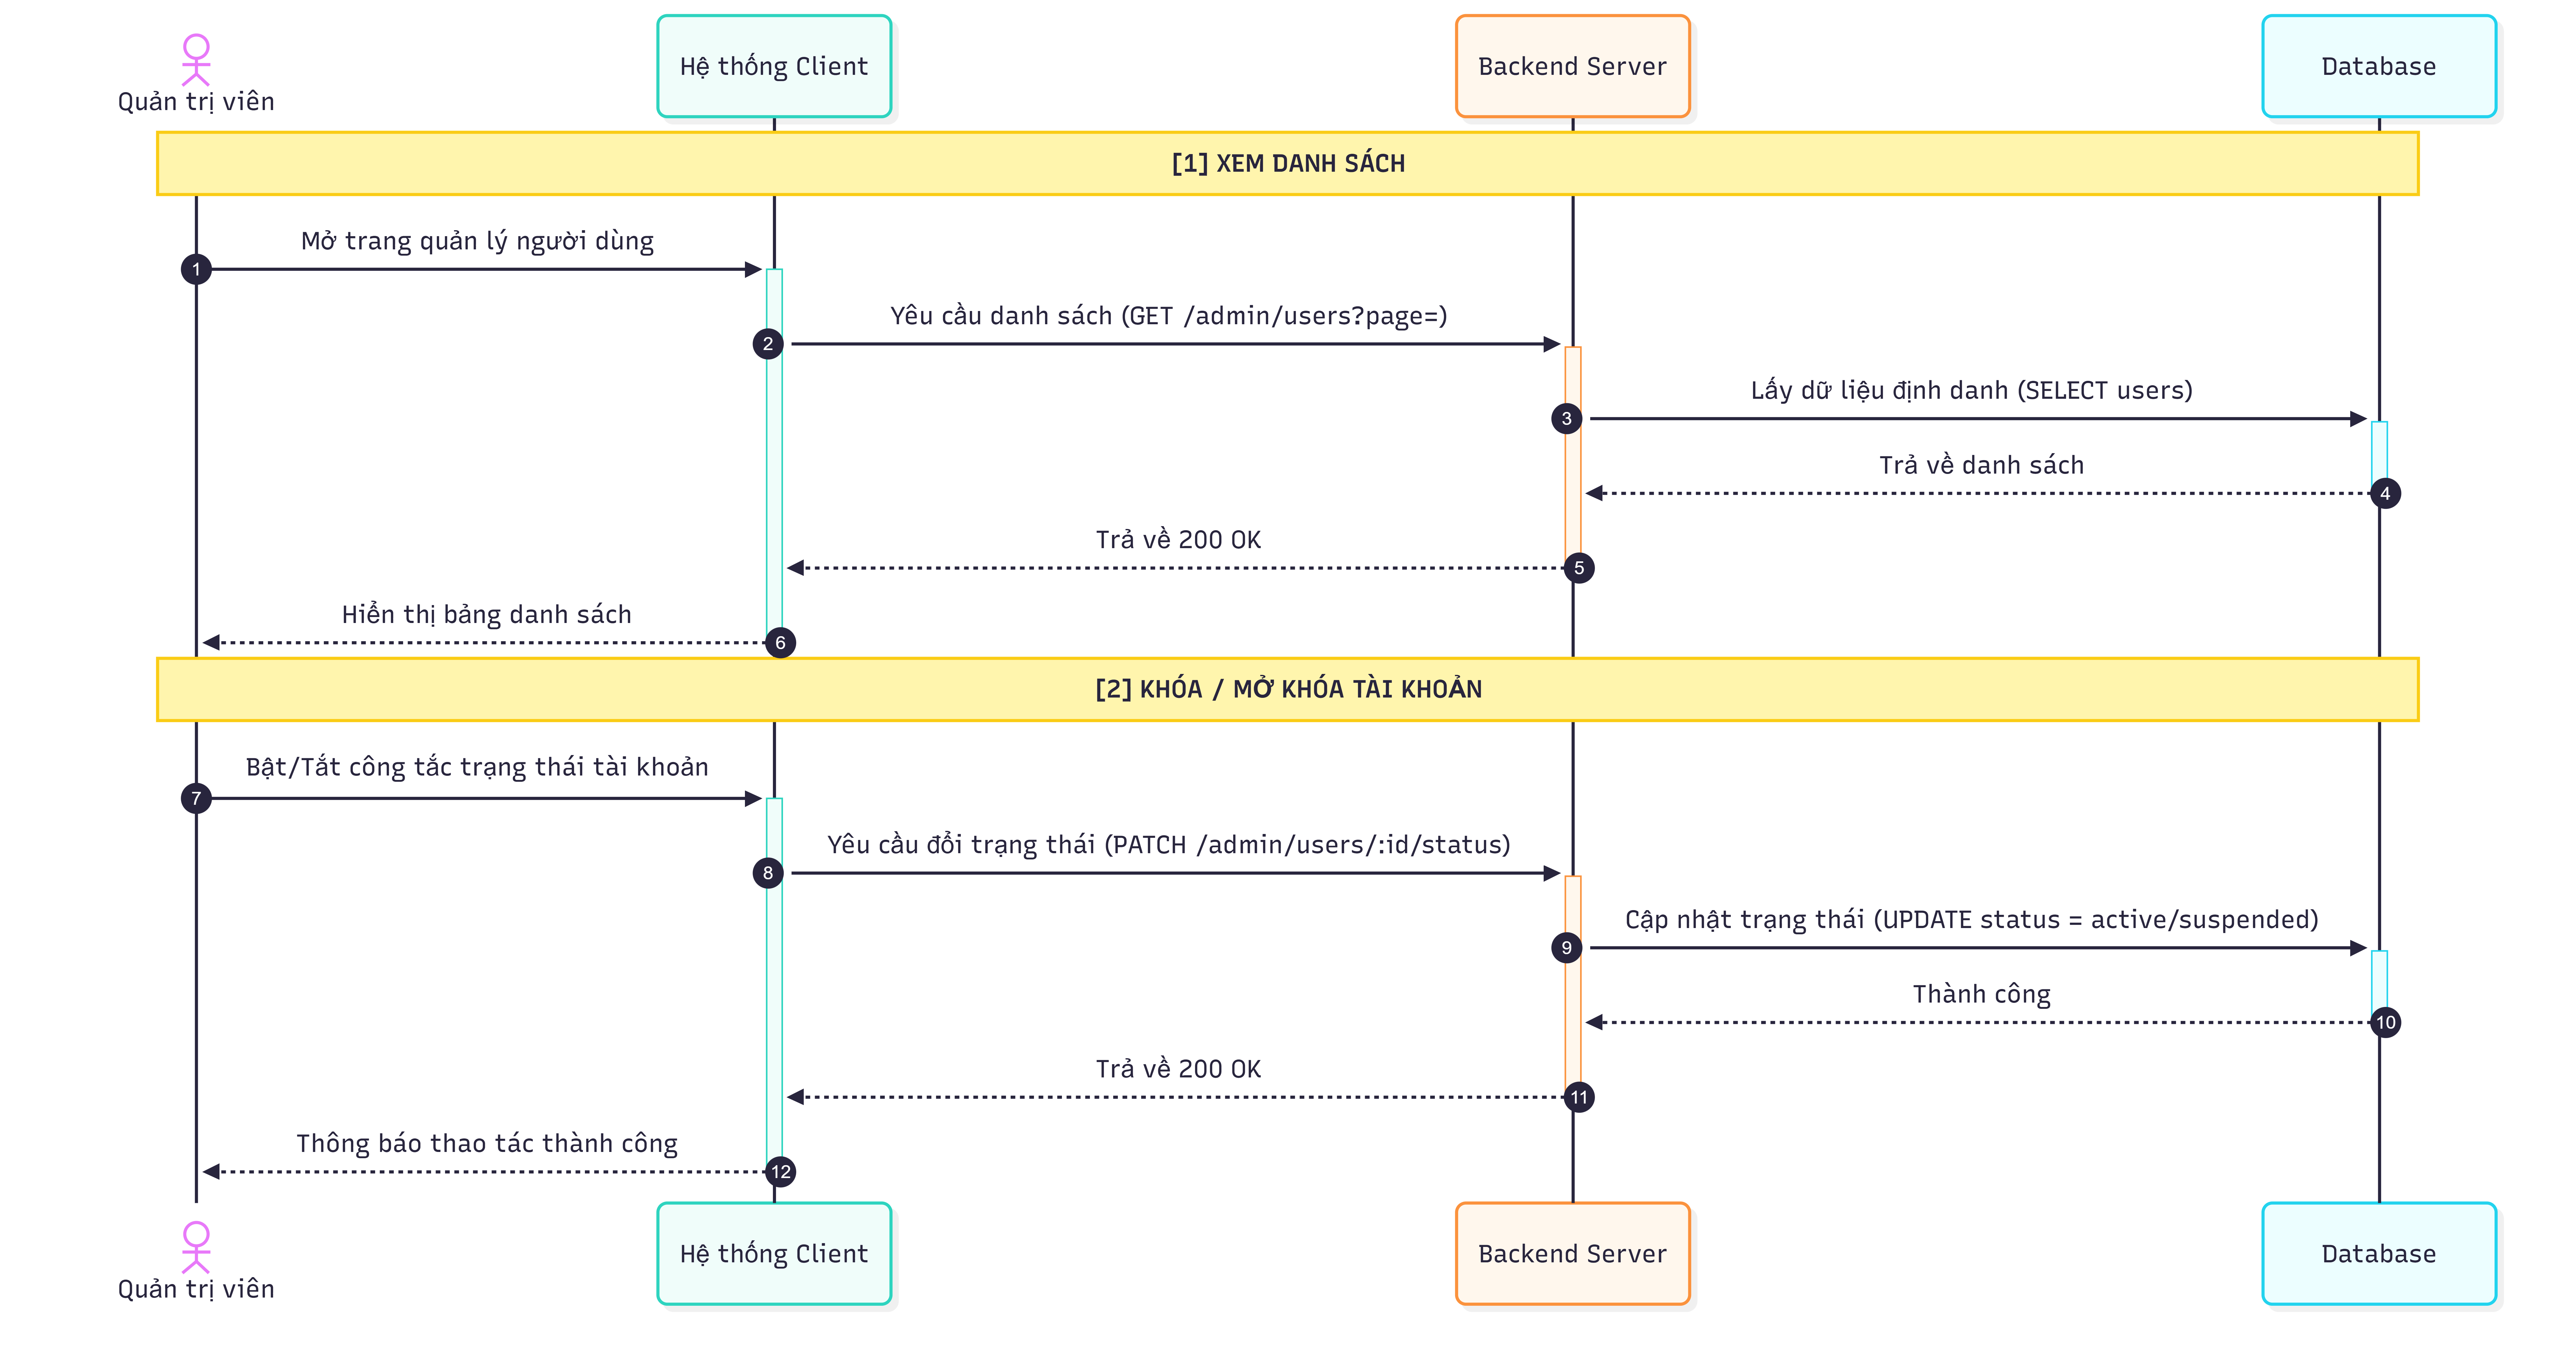
\includegraphics[width=\textwidth,height=0.85\textheight,keepaspectratio]{sd-12-user-management.png}
    \caption{Biểu đồ tuần tự: Quản lý người dùng}
    \label{fig:sd-12}
\end{figure}

\subsection{SD-13: Xử lý phản hồi (Admin)}
% \noindent\textit{[Chèn ảnh SD-13 tại đây]}
\begin{figure}[htbp]
    \centering
    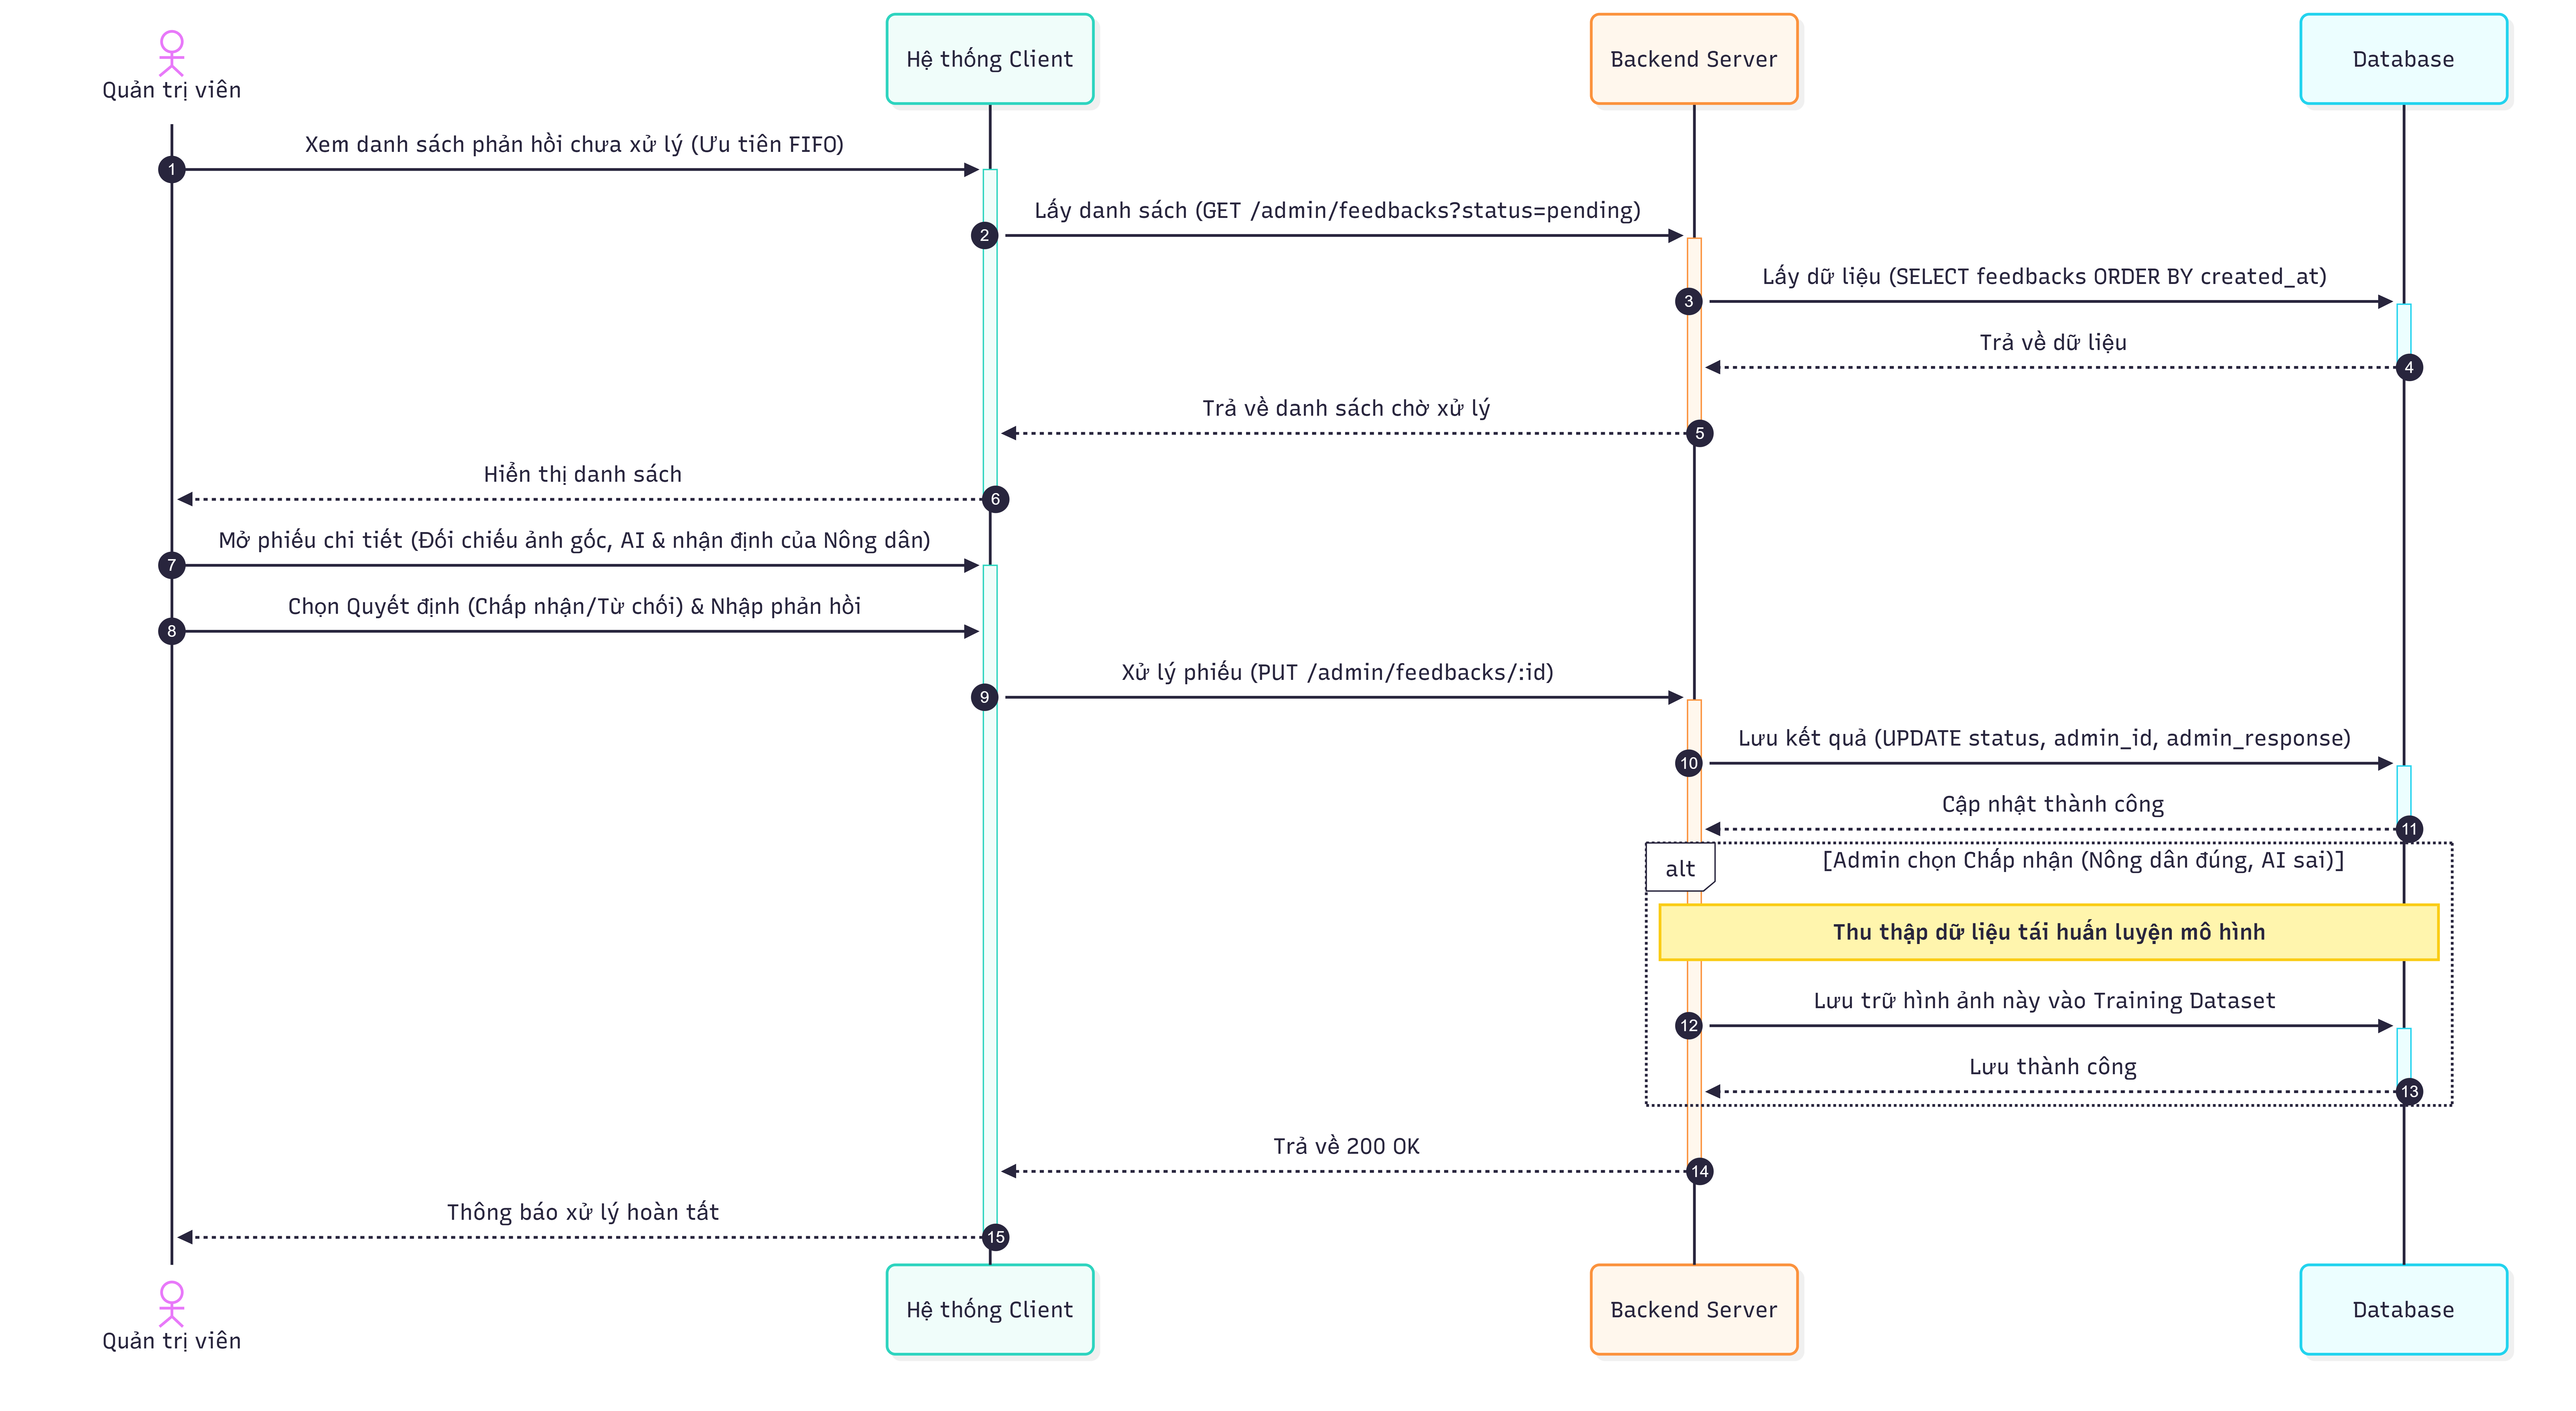
\includegraphics[width=\textwidth,height=0.85\textheight,keepaspectratio]{sd-13-feedback-admin.png}
    \caption{Biểu đồ tuần tự: Xử lý phản hồi (Admin)}
    \label{fig:sd-13}
\end{figure}

\subsection{SD-14: Cập nhật mô hình AI}
% \noindent\textit{[Chèn ảnh SD-14 tại đây]}
\begin{figure}[htbp]
    \centering
    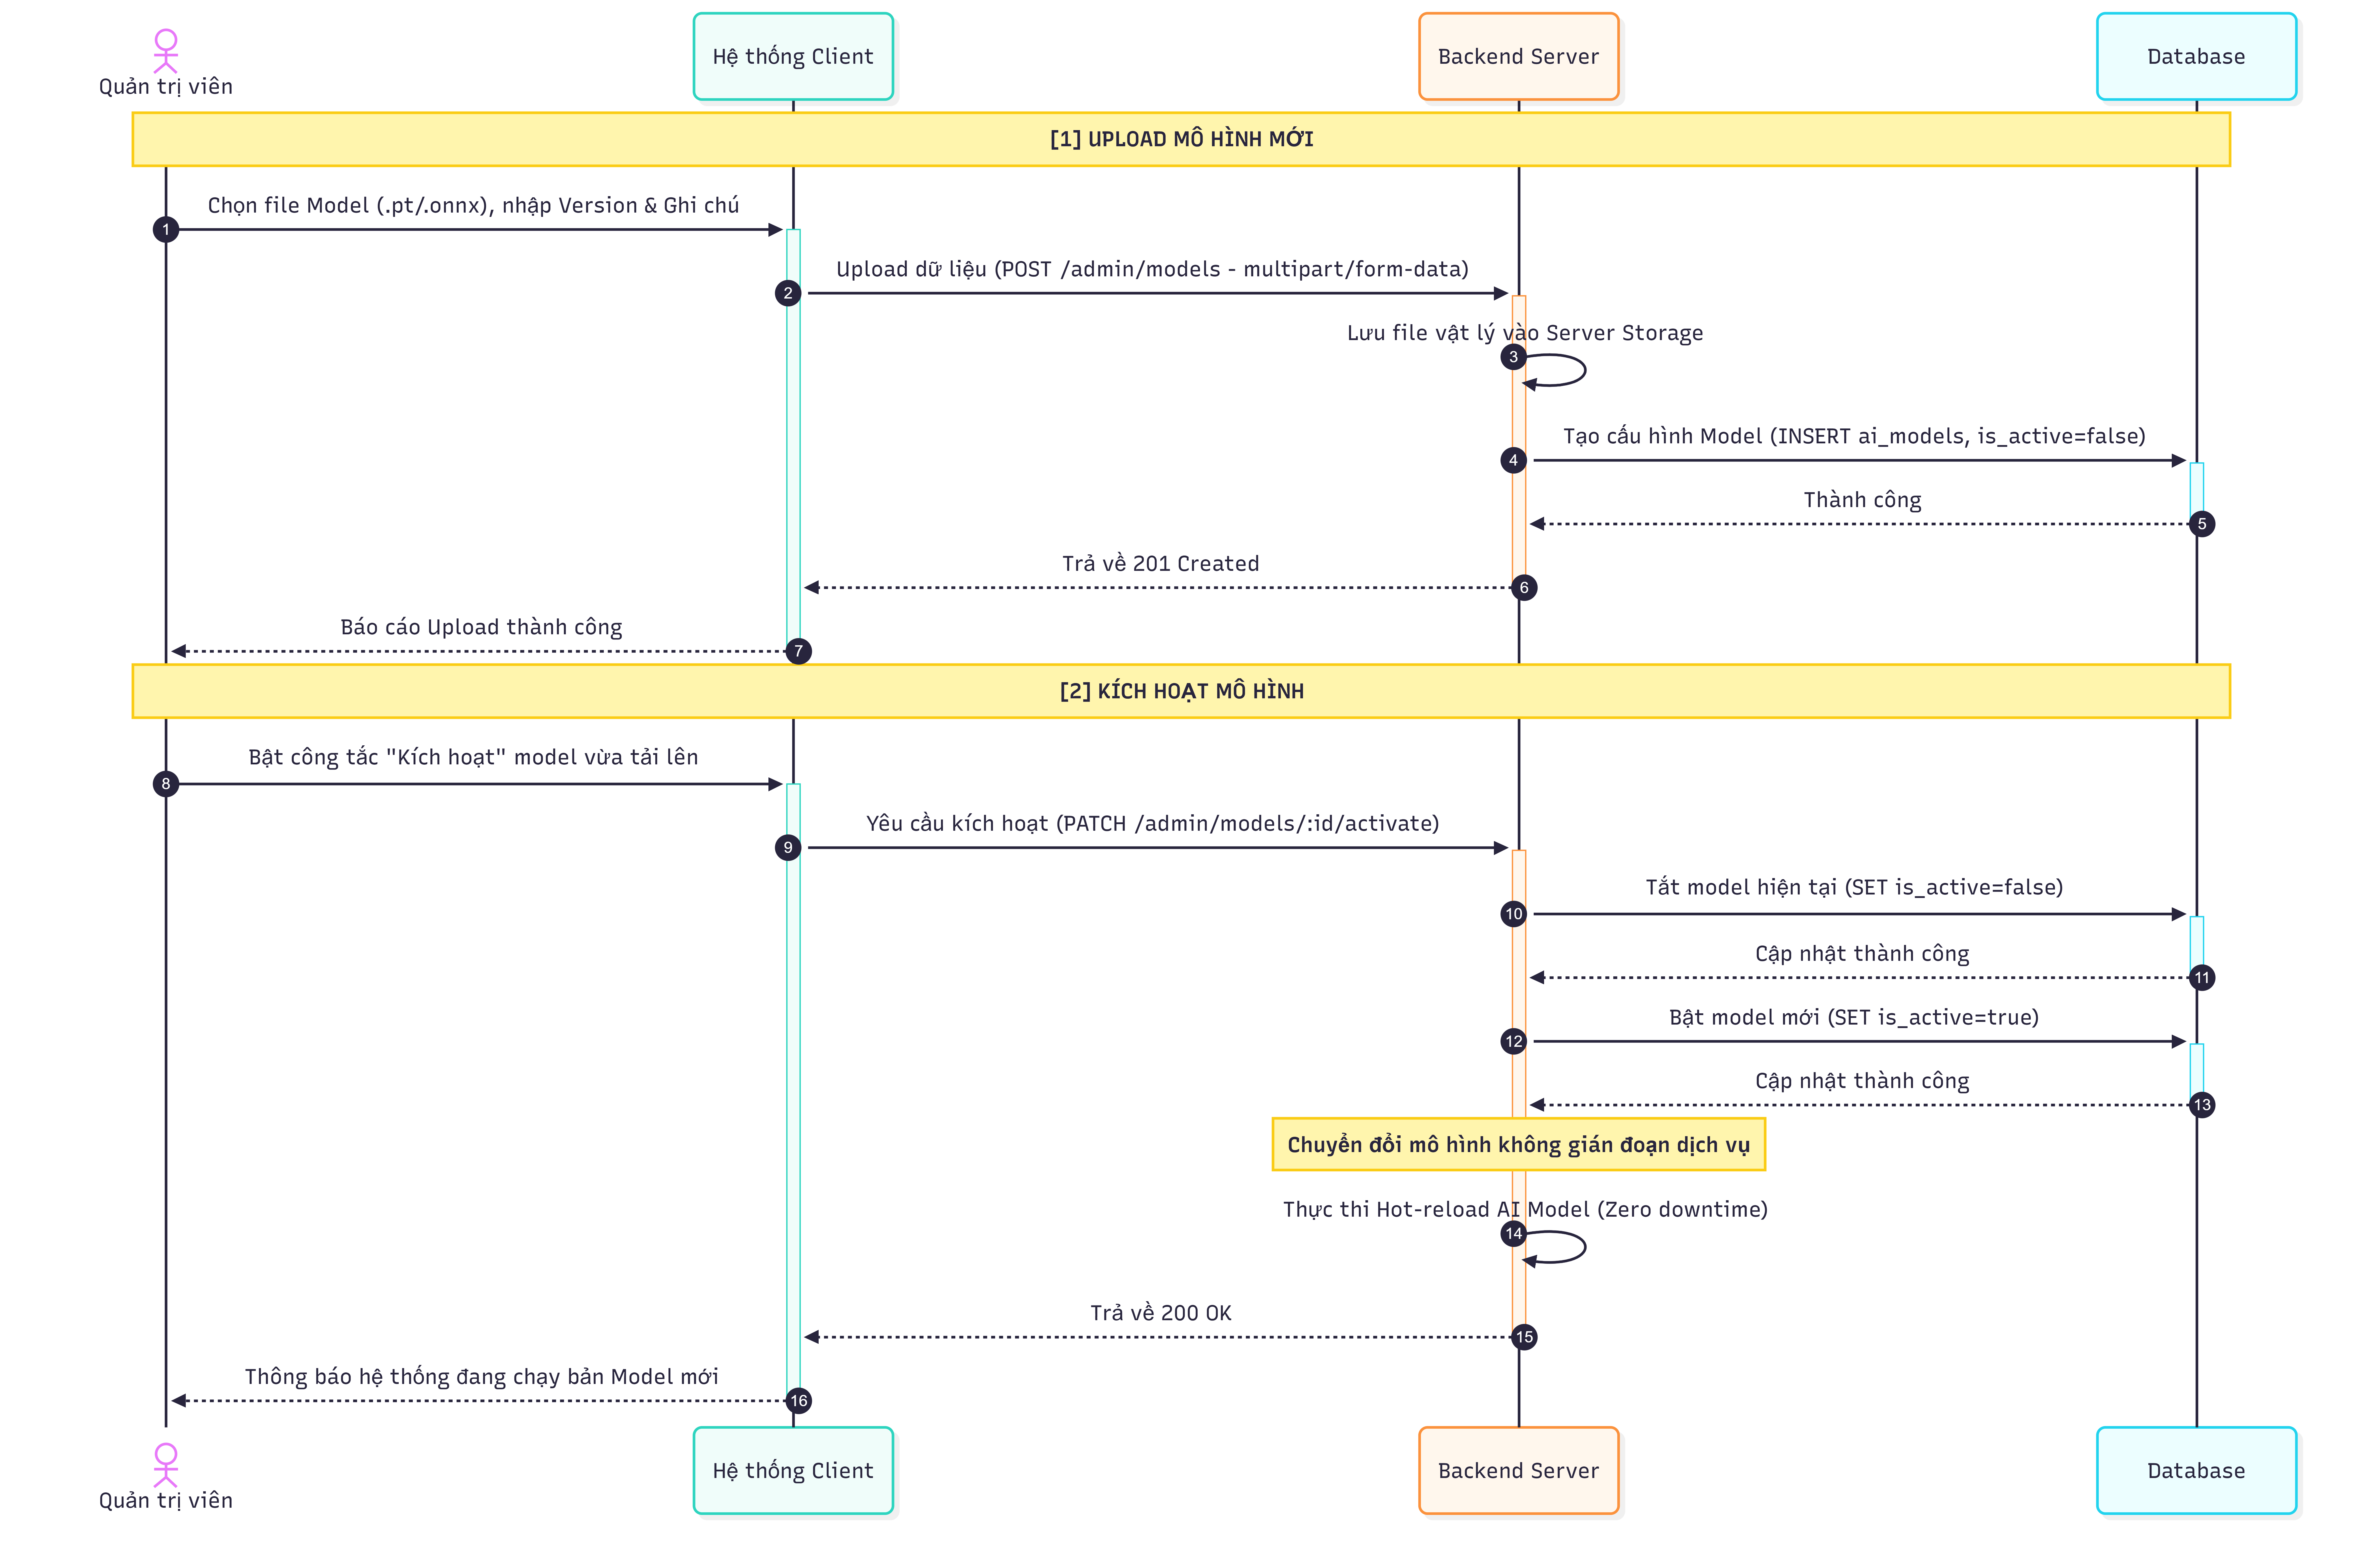
\includegraphics[width=\textwidth,height=0.85\textheight,keepaspectratio]{sd-14-model-update.png}
    \caption{Biểu đồ tuần tự: Cập nhật mô hình AI}
    \label{fig:sd-14}
\end{figure}

\subsection{SD-15: Thống kê \& Báo cáo}
% \noindent\textit{[Chèn ảnh SD-15 tại đây]}
\begin{figure}[htbp]
    \centering
    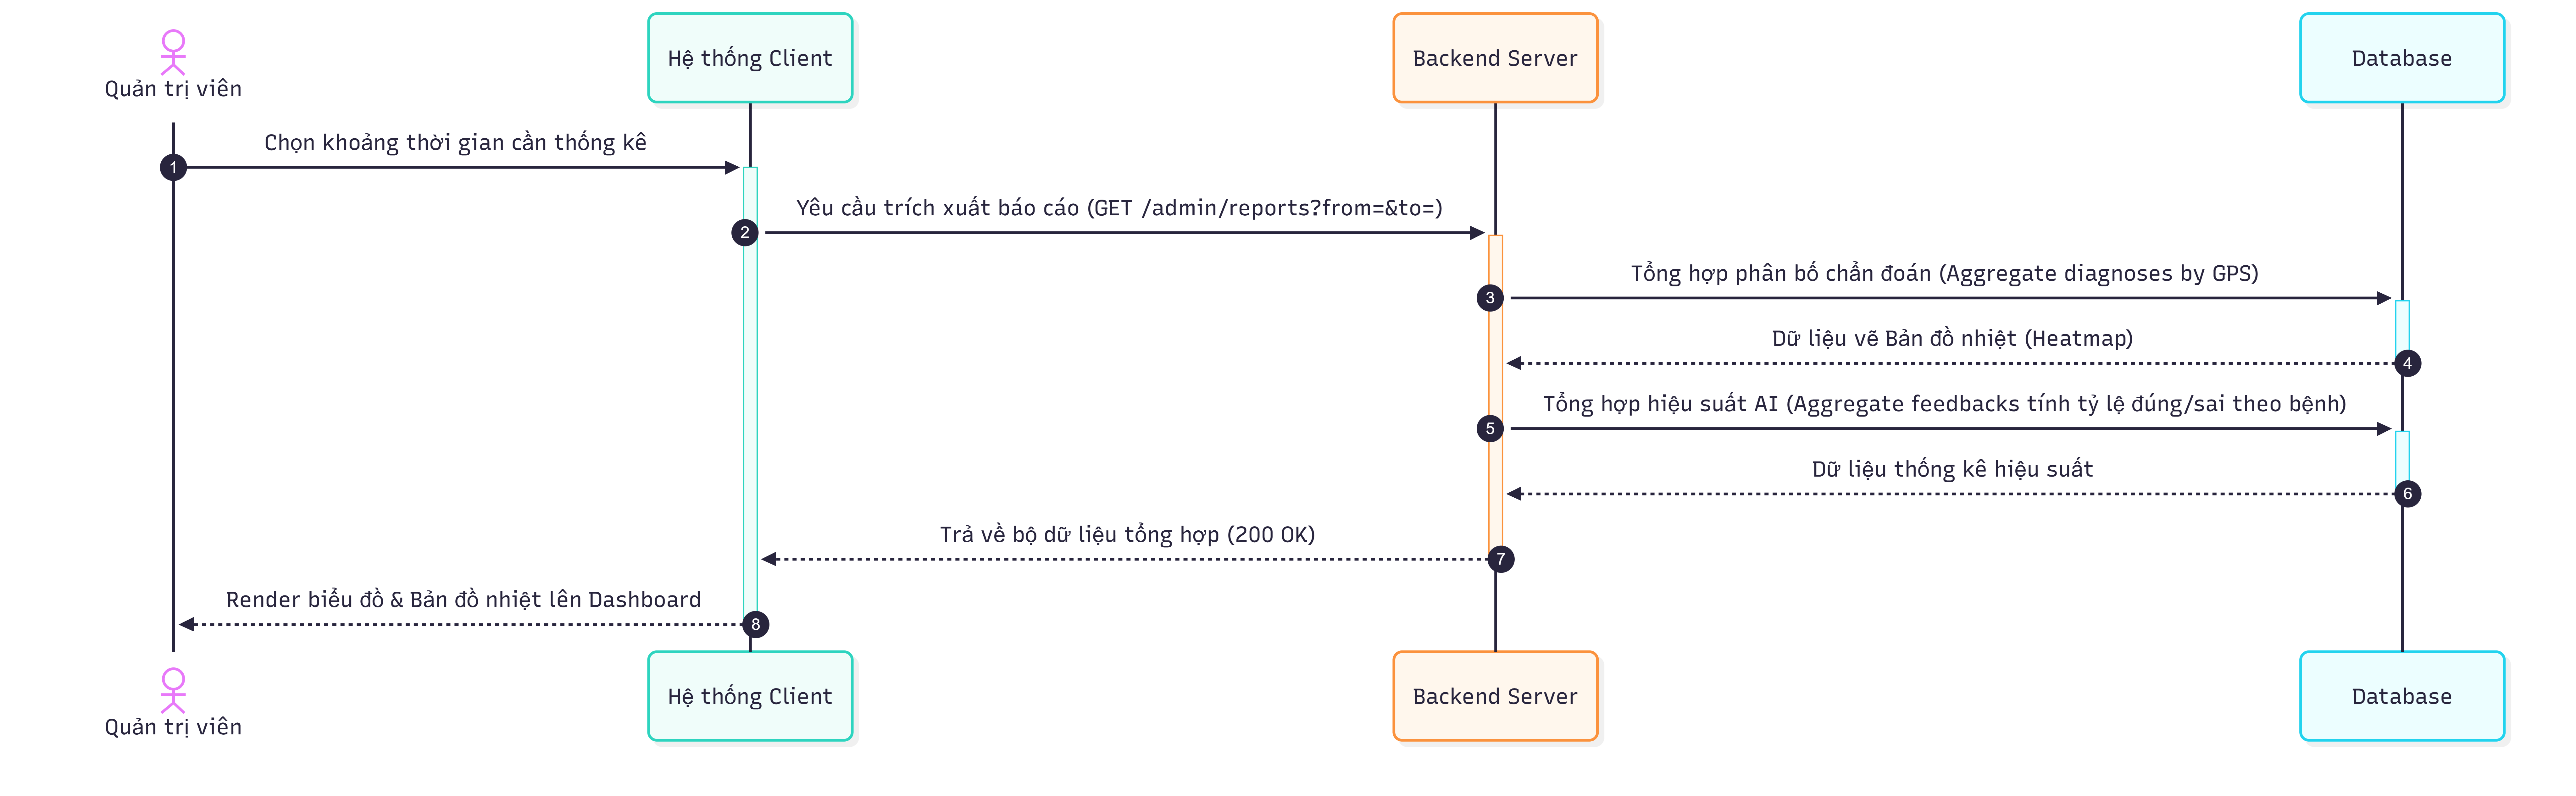
\includegraphics[width=\textwidth,height=0.85\textheight,keepaspectratio]{sd-15-reports.png}
    \caption{Biểu đồ tuần tự: Thống kê và báo cáo}
    \label{fig:sd-15}
\end{figure}

\hrulefill

% ============================================================
\section{Thiết kế Cơ sở dữ liệu}

\subsection{Bảng users}
\begin{longtable}{|l|l|l|p{5cm}|}
    \caption{Cấu trúc bảng users}                                                          \\
    \hline
    \rowcolor{headerblue}
    \textbf{Trường} & \textbf{Kiểu} & \textbf{Ràng buộc}                & \textbf{Ghi chú} \\
    \hline
    id              & UUID          & PK                                &                  \\
    \hline
    username        & VARCHAR(50)   & UNIQUE, NOT NULL                  &                  \\
    \hline
    email           & VARCHAR(255)  & UNIQUE, NOT NULL                  &                  \\
    \hline
    password\_hash  & VARCHAR(60)   & NOT NULL                          &                  \\
    \hline
    role            & ENUM          & 'user', 'admin'                   &                  \\
    \hline
    status          & ENUM          & 'active', 'inactive', 'suspended' &                  \\
    \hline
    created\_at     & TIMESTAMP     & Default now()                     &                  \\
    \hline
\end{longtable}

\textit{Lưu ý:} Số lần đăng nhập sai và thời gian khóa tạm thời được lưu trên \textbf{Redis}, không lưu trong CSDL.

\subsection{Bảng user\_profiles}
\begin{longtable}{|l|l|l|p{5.5cm}|}
    \caption{Cấu trúc bảng user\_profiles}                                                            \\
    \hline
    \rowcolor{headerblue}
    \textbf{Trường} & \textbf{Kiểu} & \textbf{Ràng buộc}             & \textbf{Ghi chú}               \\
    \hline
    id              & UUID          & PK                             &                                \\
    \hline
    user\_id        & FK            & $\rightarrow$ users.id, UNIQUE & Quan hệ 1--1                   \\
    \hline
    display\_name   & NVARCHAR(100) &                                & Họ tên hiển thị                \\
    \hline
    gps\_lat        & DECIMAL(10,8) &                                & Vĩ độ mặc định (-90 to 90)     \\
    \hline
    gps\_lng        & DECIMAL(11,8) &                                & Kinh độ mặc định (-180 to 180) \\
    \hline
    updated\_at     & TIMESTAMP     & Default now()                  &                                \\
    \hline
\end{longtable}

\subsection{Bảng diseases}
\begin{longtable}{|l|l|l|p{5.5cm}|}
    \caption{Cấu trúc bảng diseases}                                          \\
    \hline
    \rowcolor{headerblue}
    \textbf{Trường}  & \textbf{Kiểu} & \textbf{Ràng buộc}  & \textbf{Ghi chú} \\
    \hline
    id               & UUID          & PK                  &                  \\
    \hline
    name             & NVARCHAR(100) & UNIQUE, NOT NULL    & Tên tiếng Việt   \\
    \hline
    scientific\_name & VARCHAR(150)  & UNIQUE              & Tên khoa học     \\
    \hline
    signs            & TEXT          &                     & Dấu hiệu bệnh    \\
    \hline
    status           & ENUM          & 'visible', 'hidden' &                  \\
    \hline
    created\_at      & TIMESTAMP     & Default now()       &                  \\
    \hline
    updated\_at      & TIMESTAMP     &                     &                  \\
    \hline
\end{longtable}

\subsection{Bảng nutrition\_documents (Vector Database)}
\begin{longtable}{|l|l|l|p{5.5cm}|}
    \caption{Cấu trúc bảng nutrition\_documents}                                               \\
    \hline
    \rowcolor{headerblue}
    \textbf{Trường} & \textbf{Kiểu} & \textbf{Ràng buộc} & \textbf{Ghi chú}                    \\
    \hline
    id              & UUID          & PK                 &                                     \\
    \hline
    content         & TEXT          & NOT NULL           & Nội dung tri thức                   \\
    \hline
    source          & NVARCHAR(100) &                    & Nguồn tài liệu                      \\
    \hline
    embedding       & VECTOR(1536)  &                    & Vector ngữ nghĩa (pgvector)         \\
    \hline
    chunk\_metadata & JSONB         &                    & Thông tin bổ sung, hỗ trợ GIN Index \\
    \hline
    created\_at     & TIMESTAMP     & Default now()      &                                     \\
    \hline
\end{longtable}

\subsection{Bảng diagnoses}
\begin{longtable}{|l|l|l|p{5.5cm}|}
    \caption{Cấu trúc bảng diagnoses}                                                             \\
    \hline
    \rowcolor{headerblue}
    \textbf{Trường}      & \textbf{Kiểu} & \textbf{Ràng buộc}          & \textbf{Ghi chú}         \\
    \hline
    id                   & UUID          & PK                          &                          \\
    \hline
    user\_id             & FK            & $\rightarrow$ users.id      &                          \\
    \hline
    original\_image\_url & VARCHAR(512)  & NOT NULL                    &                          \\
    \hline
    result\_image\_url   & VARCHAR(512)  &                             &                          \\
    \hline
    gps\_lat             & DECIMAL(10,8) &                             & Tọa độ gọi API thời tiết \\
    \hline
    gps\_lng             & DECIMAL(11,8) &                             &                          \\
    \hline
    weather\_data        & JSONB         &                             & Dữ liệu thời tiết từ API \\
    \hline
    env\_description     & TEXT          &                             &                          \\
    \hline
    model\_version\_id   & FK            & $\rightarrow$ ai\_models.id &                          \\
    \hline
    created\_at          & TIMESTAMP     & Default now()               &                          \\
    \hline
\end{longtable}

\subsection{Bảng diagnosis\_results (1--N)}
\begin{longtable}{|l|l|l|p{6cm}|}
    \caption{Cấu trúc bảng diagnosis\_results}                                               \\
    \hline
    \rowcolor{headerblue}
    \textbf{Trường} & \textbf{Kiểu} & \textbf{Ràng buộc}         & \textbf{Ghi chú}          \\
    \hline
    id              & UUID          & PK                         &                           \\
    \hline
    diagnosis\_id   & FK            & $\rightarrow$ diagnoses.id &                           \\
    \hline
    disease\_id     & FK            & $\rightarrow$ diseases.id  &                           \\
    \hline
    confidence      & DECIMAL(5,2)  & 0--100.00                  & \% độ tin cậy             \\
    \hline
    mask\_polygon   & JSONB         &                            & Tọa độ polygon dạng JSONB \\
    \hline
\end{longtable}

\subsection{Bảng feedbacks}
\begin{longtable}{|l|l|l|p{6.5cm}|}
    \caption{Cấu trúc bảng feedbacks}                                                            \\
    \hline
    \rowcolor{headerblue}
    \textbf{Trường} & \textbf{Kiểu} & \textbf{Ràng buộc}                & \textbf{Ghi chú}       \\
    \hline
    id              & UUID          & PK                                &                        \\
    \hline
    diagnosis\_id   & FK            & $\rightarrow$ diagnoses.id        &                        \\
    \hline
    user\_id        & FK            & $\rightarrow$ users.id            & Người gửi              \\
    \hline
    user\_message   & TEXT          &                                   & Lời nhắn nông dân      \\
    \hline
    status          & ENUM          & 'pending', 'accepted', 'rejected' &                        \\
    \hline
    admin\_id       & FK            & $\rightarrow$ users.id, nullable  & Admin xử lý            \\
    \hline
    admin\_response & TEXT          &                                   & Lời nhắn admin gửi lại \\
    \hline
    processed\_at   & TIMESTAMP     &                                   &                        \\
    \hline
    created\_at     & TIMESTAMP     & Default now()                     &                        \\
    \hline
\end{longtable}

\subsection{Bảng feedback\_actual\_diseases (Junction)}
\begin{longtable}{|l|l|l|l|}
    \caption{Cấu trúc bảng feedback\_actual\_diseases}                                \\
    \hline
    \rowcolor{headerblue}
    \textbf{Trường} & \textbf{Kiểu} & \textbf{Ràng buộc} & \textbf{Ghi chú}           \\
    \hline
    feedback\_id    & UUID          & PK, FK             & $\rightarrow$ feedbacks.id \\
    \hline
    disease\_id     & UUID          & PK, FK             & $\rightarrow$ diseases.id  \\
    \hline
\end{longtable}

\subsection{Bảng ai\_models}
\begin{longtable}{|l|l|l|p{5.5cm}|}
    \caption{Cấu trúc bảng ai\_models}                                          \\
    \hline
    \rowcolor{headerblue}
    \textbf{Trường} & \textbf{Kiểu} & \textbf{Ràng buộc}     & \textbf{Ghi chú} \\
    \hline
    id              & UUID          & PK                     &                  \\
    \hline
    version\_name   & NVARCHAR(50)  & NOT NULL               & Tên phiên bản    \\
    \hline
    file\_path      & VARCHAR(512)  & NOT NULL               & Đường dẫn file   \\
    \hline
    release\_notes  & TEXT          &                        & Ghi chú thay đổi \\
    \hline
    is\_active      & BOOLEAN       & Default false          & Chỉ 1 active     \\
    \hline
    uploaded\_by    & FK            & $\rightarrow$ users.id & Admin upload     \\
    \hline
    created\_at     & TIMESTAMP     & Default now()          &                  \\
    \hline
    updated\_at     & TIMESTAMP     &                        &                  \\
    \hline
\end{longtable}

\subsection{Redis Keys}
\begin{longtable}{|l|p{7.5cm}|l|}
    \caption{Các pattern key trong Redis}                                              \\
    \hline
    \rowcolor{headerblue}
    \textbf{Key Pattern}    & \textbf{Mô tả}        & \textbf{TTL}                     \\
    \hline
    login:fail:\{username\} & Số lần đăng nhập sai  & 15 phút (user) / 30 phút (admin) \\
    \hline
    otp:\{email\}           & OTP 6 số + số lần thử & 10 phút                          \\
    \hline
    verify:\{token\}        & Token xác thực email  & 24 giờ                           \\
    \hline
\end{longtable}

\subsection{Sơ đồ quan hệ thực thể (ERD)}

% \noindent\textit{[Chèn ảnh ER Diagram tại đây --- sinh từ db.dbml]}
\begin{figure}[htbp]
    \centering
    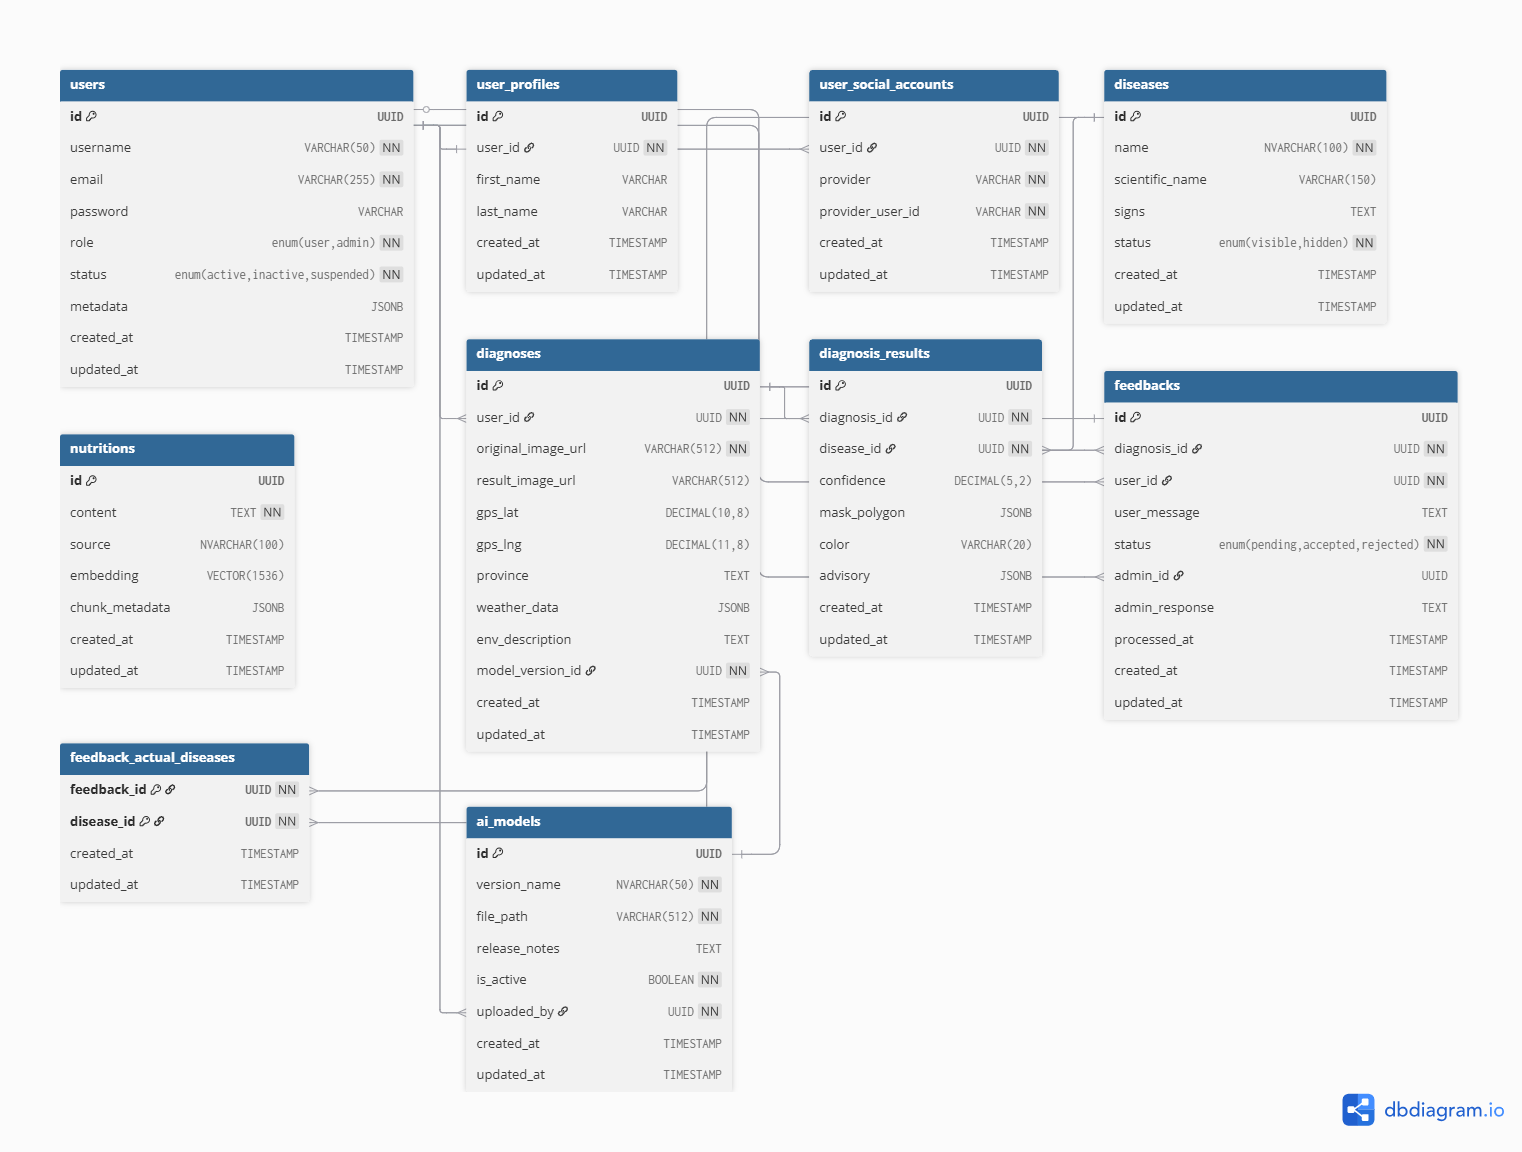
\includegraphics[width=\textwidth,height=0.85\textheight,keepaspectratio]{erd.png}
    \caption{Sơ đồ quan hệ thực thể (ERD)}
    \label{fig:erd}
\end{figure}

\hrulefill

% ============================================================
\section{Giải thích thuật ngữ}

\begin{longtable}{|l|p{11.5cm}|}
    \caption{Giải thích các thuật ngữ chuyên ngành}                                                           \\
    \hline
    \rowcolor{headerblue}
    \textbf{Thuật ngữ}    & \textbf{Giải thích}                                                               \\
    \hline
    CNN                   & Mạng nơ-ron tích chập --- thuật toán AI chuyên phân tích hình ảnh.                \\
    \hline
    Instance Segmentation & Kỹ thuật AI khoanh vùng chính xác từng đối tượng bệnh trên ảnh (pixel-level).     \\
    \hline
    pgvector              & Phần mở rộng của PostgreSQL cho phép tìm kiếm ngữ nghĩa trên dữ liệu văn bản.     \\
    \hline
    Embedding             & Biểu diễn số của văn bản để máy hiểu nghĩa, phục vụ tìm kiếm thông minh.          \\
    \hline
    RAG                   & Retrieval-Augmented Generation --- truy xuất tri thức để AI tư vấn chính xác hơn. \\
    \hline
    Redis                 & Bộ nhớ đệm tốc độ cao, dùng lưu tạm OTP và đếm lần đăng nhập sai.                 \\
    \hline
    JWT                   & Mã thông báo xác thực, giữ trạng thái đăng nhập của người dùng.                   \\
    \hline
    Bcrypt                & Thuật toán mã hóa mật khẩu một chiều, không thể giải ngược.                       \\
    \hline
    OTP                   & Mã xác thực dùng một lần, gửi qua email, hết hạn sau 10 phút.                     \\
    \hline
    GPS                   & Hệ thống định vị toàn cầu, xác định tọa độ vị trí người dùng.                     \\
    \hline
    Hot-swap              & Thay thế mô hình AI mà không cần tắt hệ thống.                                    \\
    \hline
    ERD                   & Sơ đồ thực thể quan hệ --- mô tả cấu trúc và quan hệ giữa các bảng dữ liệu.       \\
    \hline
    mask\_polygon         & Mảng tọa độ đa giác mô tả đường viền vùng bệnh trên ảnh.                          \\
    \hline
\end{longtable}

\end{document}
